%====================================================================
% NUTAN MAHARASHTRA VIDYA PRASARAK MANDAL'S
% NUTAN COLLEGE OF ENGINEERING & RESEARCH (NCER)
% Department of Computer Science and Engineering
% Project Report - Phase I - 2025-26
% Title: CAUSALYTIX - Engineering Workspace for Investigating
%        Software and Hardware Failures
%
% Complies with: Project Report Guidelines 2025-26
%   - A4, Times New Roman, Heading 16 Bold, Subheading 14 Bold, Normal 12
%   - Line spacing 1.5, Margins L1.5in R1in T1in B1in
%   - Page numbers at right bottom, continuous
%   - Header right: Project Title, Footer left: Department name
%   - Index as per Project Phase I Index Format.pdf
%
% Author names / PRN / Mentor / Coordinator left BLANK for later insertion
% 40 research papers are cited and listed in references.bib (IEEE style)
%====================================================================

\documentclass[12pt,a4paper,oneside]{report}

% ---------- Page geometry (Guideline #5) ----------
\usepackage[
  a4paper,
  left=1.5in,
  right=1in,
  top=1in,
  bottom=1in,
  headheight=14pt,
  footskip=28pt
]{geometry}

% ---------- Fonts: Times New Roman ----------
\usepackage{times}               % Times clone for pdflatex
\usepackage{newtxtext,newtxmath} % better Times
\usepackage[T1]{fontenc}
\usepackage[utf8]{inputenc}

% ---------- Language & spacing ----------
\usepackage[english]{babel}
\usepackage{setspace}
\onehalfspacing                 % 1.5 line spacing (Guideline #4)
\usepackage{parskip}
\setlength{\parskip}{0.5em}
\setlength{\parindent}{1.25em}
\usepackage{microtype}

% ---------- Headings: 16 Bold, 14 Bold (Guideline #3) ----------
\usepackage{titlesec}
\titleformat{\chapter}[display]
  {\normalfont\fontsize{16}{19}\bfseries\color{black}}
  {\chaptertitlename\ \thechapter}
  {6pt}
  {\fontsize{16}{19}\bfseries}
  [\vspace{6pt}\hrule\vspace{8pt}]
\titlespacing*{\chapter}{0pt}{0pt}{10pt}

\titleformat{\section}
  {\normalfont\fontsize{14}{17}\bfseries}
  {\thesection}{0.6em}{}
\titlespacing*{\section}{0pt}{12pt}{6pt}

\titleformat{\subsection}
  {\normalfont\fontsize{13}{15}\bfseries}
  {\thesubsection}{0.6em}{}
\titlespacing*{\subsection}{0pt}{10pt}{4pt}

\titleformat{\subsubsection}
  {\normalfont\fontsize{12}{14}\bfseries\itshape}
  {\thesubsubsection}{0.6em}{}

% ---------- Header / Footer (Guideline #7) ----------
\usepackage{fancyhdr}
\usepackage{xcolor}
\definecolor{ncerTeal}{HTML}{0e2927}
\definecolor{ncerLight}{HTML}{117664}
\pagestyle{fancy}
\fancyhf{}
% Header: Right side Project Title
\fancyhead[R]{\small\textit{Causalytix --- From Symptom to Cause}}
\renewcommand{\headrulewidth}{0.6pt}
\renewcommand{\headrule}{\hbox to\headwidth{\color{ncerLight}\leaders\hrule height \headrulewidth\hfill}}
% Footer: Left Dept, Right Page Number (Guideline #6 + #7)
\fancyfoot[L]{\footnotesize Department of CSE, Nutan College of Engineering and Research, Talegaon, Pune}
\fancyfoot[R]{\footnotesize \thepage}
\fancypagestyle{plain}{
  \fancyhf{}
  \fancyfoot[L]{\footnotesize Department of CSE, Nutan College of Engineering and Research, Talegaon, Pune}
  \fancyfoot[R]{\footnotesize \thepage}
  \renewcommand{\headrulewidth}{0pt}
}

% ---------- Figures, Tables, Captions ----------
\usepackage{graphicx}
\graphicspath{{images/}{../public/assets/atlas/}}
\usepackage{caption}
\usepackage{subcaption}
\captionsetup{font=small,labelfont=bf,skip=6pt}
\usepackage{float}
\usepackage{booktabs}
\usepackage{longtable}
\usepackage{array}
\usepackage{multirow}
\usepackage{tabularx}
\usepackage{lscape}
\usepackage{pdflscape}
\usepackage{enumitem}
\setlist[itemize]{leftmargin=1.8em}
\setlist[enumerate]{leftmargin=1.8em}

% ---------- Math & symbols ----------
\usepackage{amsmath,amssymb,amsthm}

% ---------- Hyperlinks ----------
\usepackage[hidelinks,bookmarksnumbered,bookmarksopen=true]{hyperref}
\hypersetup{
  colorlinks=false,
  linkbordercolor=white,
  pdfauthor={NCER CSE - Causalytix Team},
  pdftitle={Causalytix Project Report Phase-I 2025-26},
  pdfsubject={Root Cause Analysis Workspace}
}

% ---------- Bibliography ----------
\usepackage[numbers,sort&compress]{natbib}
\usepackage{url}
\usepackage{etoolbox}

% ---------- TOC depth ----------
\setcounter{secnumdepth}{3}
\setcounter{tocdepth}{3}

% ---------- Custom commands ----------
\newcommand{\projecttitle}{Causalytix: Engineering Workspace for Investigating Software and Hardware Failures}
\newcommand{\deptfooter}{Department of CSE, Nutan College of Engineering and Research, Talegaon, Pune}
\newcommand{\blankline}[1][3cm]{\rule{#1}{0.4pt}}

\begin{document}

%====================================================================
% FRONT MATTER
%====================================================================
\pagenumbering{roman}

% ---------------- Title Page ----------------
\begin{titlepage}
\centering
\vspace*{0.2cm}
{\large \textbf{NUTAN MAHARASHTRA VIDYA PRASARAK MANDAL'S}}\par
\vspace{0.2cm}
{\Large \textbf{NUTAN COLLEGE OF ENGINEERING \& RESEARCH (NCER)}}\par
\vspace{0.1cm}
{\normalsize \textit{Department of Computer Science and Engineering}}\par
\vspace{0.1cm}
{\footnotesize Talegaon Dabhade, Pune -- 410507 $\bullet$ Approved by AICTE $\bullet$ Affiliated to Savitribai Phule Pune University}\par
\hrule\vspace{0.3cm}
\vspace{0.3cm}
% College logo placeholder — replace with \includegraphics[width=0.18\textwidth]{ncer-logo.pdf}
% Requires file report/images/ncer-logo.pdf (or .png). Placeholder box below avoids missing-file error.
\begin{center}
\fbox{\parbox{0.18\textwidth}{\centering \footnotesize \textit{NCER Logo}\\ \texttt{ncer-logo.pdf}\\ \textit{(replace placeholder)}}}
\end{center}
\vspace{0.3cm}

{\large \textbf{A PROJECT REPORT ON}}\par
\vspace{0.4cm}
{\LARGE \textbf{\projecttitle}}\par
\vspace{0.2cm}
{\large \textit{From Symptom to Cause: Ranked Hypotheses, Evidence-Linked 5-Why Chains \& Human-Verified Corrective Actions}}\par
\vspace{0.5cm}
{\normalsize \textbf{Submitted in Partial Fulfillment of the Requirements for the Degree of}}\par
\vspace{0.15cm}
{\large \textbf{Bachelor of Engineering (B.E.) in Computer Engineering}}\par
\vspace{0.15cm}
{\normalsize Academic Year 2025--26}\par
\vspace{0.6cm}

\begin{tabular}{l l}
\textit{Submitted By:} & \blankline[6cm] \quad (PRN: \blankline[4cm])\\
                       & \blankline[6cm] \quad (PRN: \blankline[4cm])\\
                       & \blankline[6cm] \quad (PRN: \blankline[4cm])\\
                       & \blankline[6cm] \quad (PRN: \blankline[4cm])\\
\end{tabular}

\vspace{0.5cm}
\begin{tabular}{l l}
\textit{Under the Guidance of:} & \blankline[6cm]\\
\textit{Project Coordinator:}    & \blankline[6cm] \quad (Prof.\ S.\ B.\ Mehta)\\
\textit{Head of Department:}     & \textbf{Dr.\ Mahesh Wankhade}\\
\end{tabular}

\vfill
{\small Savitribai Phule Pune University, Pune}\par
\vspace{0.2cm}
\end{titlepage}

% ---------------- Certificate Page ----------------
\chapter*{Certificate}
\addcontentsline{toc}{chapter}{Certificate}
\begin{center}
\textit{This is to certify that the Project Report entitled}
\end{center}
\begin{center}
{\large \textbf{\projecttitle}}\par
\end{center}
\begin{center}
\textit{has been successfully completed by}
\end{center}
\vspace{0.2cm}
\begin{center}
\begin{tabular}{l l}
 & \blankline[7cm] \quad (PRN: \blankline[4cm])\\
 & \blankline[7cm] \quad (PRN: \blankline[4cm])\\
 & \blankline[7cm] \quad (PRN: \blankline[4cm])\\
 & \blankline[7cm] \quad (PRN: \blankline[4cm])\\
\end{tabular}
\end{center}
\vspace{0.2cm}
\begin{center}
\textit{in partial fulfillment for the award of Degree of Bachelor of Engineering in Computer Engineering at}\\
\textbf{Nutan College of Engineering \& Research, Talegaon, Pune}\\
\textit{during the Academic Year 2025--26, as per the guidelines of Savitribai Phule Pune University.}
\end{center}
\vspace{0.8cm}
\noindent
\begin{tabular}{p{0.45\textwidth} p{0.45\textwidth}}
\blankline[5.5cm] & \blankline[5.5cm] \\
\textbf{Project Guide} \quad \textit{(Name to be inserted)} & \textbf{Project Coordinator} \\
 & Prof.\ S.\ B.\ Mehta \\
 & \\
\blankline[5.5cm] & \blankline[5.5cm] \\
\textbf{Head of Department} & \textbf{Principal} \\
Dr.\ Mahesh Wankhade & \textit{(Principal, NCER)} \\
Department of CSE, NCER & Nutan College of Engineering \& Research \\
 & \\
\textit{Date: \blankline[3cm]} & \textit{Place: Talegaon Dabhade, Pune} \\
\end{tabular}

\vspace{0.6cm}
\begin{flushright}
\small \textit{College Seal}
\end{flushright}

% ---------------- Declaration ----------------
\chapter*{Declaration}
\addcontentsline{toc}{chapter}{Declaration}
We, the undersigned, hereby declare that the project report entitled \textbf{\projecttitle} submitted to Savitribai Phule Pune University, Pune for the award of Bachelor of Engineering in Computer Engineering is a record of original work carried out by us under the guidance of \blankline[4cm] (Project Guide) and coordination of Prof.\ S.\ B.\ Mehta. The work has not been submitted elsewhere for any degree or diploma. All sources of information have been duly acknowledged and the 40 research papers cited have been consulted for this report.

\vspace{0.8cm}
\noindent
\begin{tabular}{l l}
Signature: & \blankline[5cm] \quad Date: \blankline[3cm]\\
Signature: & \blankline[5cm] \quad Date: \blankline[3cm]\\
Signature: & \blankline[5cm] \quad Date: \blankline[3cm]\\
Signature: & \blankline[5cm] \quad Date: \blankline[3cm]\\
\end{tabular}

% ---------------- Acknowledgement ----------------
\chapter*{Acknowledgement}
\addcontentsline{toc}{chapter}{Acknowledgement}
We express our sincere gratitude to \textbf{Dr.\ Mahesh Wankhade}, Head, Department of Computer Science and Engineering, NCER, and to our Project Coordinator \textbf{Prof.\ S.\ B.\ Mehta} for their continuous encouragement, valuable guidance and for providing the infrastructure to carry out this work.

We are deeply indebted to our Project Guide \blankline[5cm] for insightful suggestions, for introducing us to root-cause thinking (Ishikawa, 5-Whys, causal inference) and for reviewing our retrieval-plus-ranking design. We thank all faculty members of the Department of CSE for their cooperation.

We extend thanks to our families, friends and to the open-source community (FastAPI, React, Supabase, ReportLab) whose tools made \textit{Causalytix} possible. We acknowledge the 40 cited authors whose research shaped our literature survey.

\vspace{0.5cm}
\begin{flushright}
\textit{--- Project Team, B.E.\ CSE, NCER (2025--26)}
\end{flushright}

% ---------------- Abstract ----------------
\chapter*{Abstract}
\addcontentsline{toc}{chapter}{Abstract}
\noindent \textbf{Keywords:} Root Cause Analysis, Ishikawa Diagram, 5-Why Analysis, Retrieval-Augmented Generation, Evidence Matching, Incident Management, AIOps, Hardware Fault Diagnosis, Human-in-the-Loop Verification

\vspace{0.3cm}
Modern software and hardware systems fail in ways that are \textit{distributed, intermittent and multi-causal}. A gateway latency spike, a field-controller reset or a memory-leak container restart rarely has a single obvious culprit. Industry studies report that $\sim$74\% of failures are recurring \cite{wang2024comprehensive}, yet mean time to recovery (MTTR) remains dominated by manual hunting through logs, metrics, traces and bench notes.

\textbf{Causalytix} is an engineering workspace that turns a symptom into a set of \textit{ranked, testable hypotheses}. An investigator supplies a brief (observed vs.\ expected behaviour, affected system, timeline) and up to six evidence documents (logs, CSVs, markdown, JSON, text-layer PDFs or pasted bench notes). The system chunks evidence into 760-character overlapping passages, hashes each passage into a deterministic 256-dimensional log-TF vector, and stores it in a passage index. At analysis time the workspace (i) proposes 3--6 candidate root causes classified by category (Infrastructure, Configuration, Network, Runtime, Process, Environment, Power, Mechanical), (ii) expands each candidate into a five-level \textit{Why} chain, (iii) independently matches every cause and every Why statement against the current incident's passages via cosine similarity (threshold 0.20 marks ``Needs evidence''), and (iv) ranks candidates by the transparent formula \[ \text{rank}= \text{round}(100\times(0.50\cdot\text{evidence}+0.30\cdot\text{impact}+0.20\cdot\text{history})) \] where \textit{history} counts similar human-confirmed mechanisms in resolved cases of the same domain, saturating at three.

Two inference modes are supported: a \textbf{local classifier} (multinomial naive Bayes trained on labelled playbook examples with abstention for out-of-vocabulary incidents) that works offline, and an \textbf{optional language-model adapter} (two OpenAI-compatible JSON completions, validated by Pydantic) that brings RAG-style fluency without bypassing the gateway's evidence-matching and ranking. A human verification gate is required to resolve an investigation: the engineer selects the confirmed cause and records the test outcome; only that mechanism influences future history. The local SQLite database (WAL mode) is the system of record; cloud archival to Supabase (Postgres + pgvector, owner-scoped RLS) is explicit and opt-in.

The workspace delivers clickable Ishikawa (fishbone) branches, five linked Why nodes per candidate, source inspection (document, passage number, excerpt), separation of containment / prevention / verification, and export of a paginated PDF or machine-readable JSON. Eleven architecture and workflow diagrams are provided for the project report. Phase-I demonstrates the full nine-stage workflow on eight illustrative starter cases and passes isolated SQLite + API + inference tests, including WASM-based PostgreSQL policy tests.

% ---------------- TOC / LOF / LOT / LOA ----------------
\tableofcontents
\listoffigures
\addcontentsline{toc}{chapter}{List of Figures}
\listoftables
\addcontentsline{toc}{chapter}{List of Tables}

\chapter*{List of Abbreviations}
\addcontentsline{toc}{chapter}{List of Abbreviations}
\begin{longtable}{p{2.8cm} p{11.5cm}}
\toprule
\textbf{Abbreviation} & \textbf{Description}\\
\midrule
RCA & Root Cause Analysis\\
AIOps & Artificial Intelligence for IT Operations\\
LLM & Large Language Model\\
RAG & Retrieval-Augmented Generation\\
TF & Term Frequency\\
BM25 & Best Matching 25 (probabilistic retrieval model)\\
MTTR & Mean Time To Recovery\\
MTBF & Mean Time Between Failures\\
MTTF & Mean Time To Failure\\
ERD & Entity Relationship Diagram\\
API & Application Programming Interface\\
SPA & Single Page Application\\
WAL & Write-Ahead Logging (SQLite)\\
RLS & Row Level Security (PostgreSQL)\\
JWT & JSON Web Token\\
UI & User Interface\\
SVG & Scalable Vector Graphics\\
PDF & Portable Document Format\\
JSON & JavaScript Object Notation\\
CSV & Comma-Separated Values\\
CPU & Central Processing Unit\\
OOM & Out Of Memory\\
DNS & Domain Name System\\
CI/CD & Continuous Integration / Continuous Delivery\\
CAPA & Corrective and Preventive Action\\
FMEA & Failure Mode and Effects Analysis\\
8D & Eight Disciplines of Problem Solving\\
KQL & Kusto Query Language\\
PG & PostgreSQL\\
\bottomrule
\end{longtable}

%====================================================================
% MAIN MATTER - PAGE NUMBERING RESTARTS AT 1 (continuous per guideline)
%====================================================================
\cleardoublepage
\pagenumbering{arabic}
\setcounter{page}{1}

%====================================================================
% CHAPTER 1 - INTRODUCTION
%====================================================================
\chapter{Introduction}
\label{ch:intro}

\section{Introduction}
\label{sec:intro}

Software no longer runs on a single machine and hardware no longer fails with a simple burnt fuse. A typical student project, a campus SaaS deployment or a factory field-controller now spans browsers, gateways, queues, orchestrators, firmware, power delivery and human operators. When a symptom appears --- ``API gateway latency spikes with database pool wait timeouts'' or ``controller resets when load starts with a time-aligned voltage dip'' --- the true cause can hide several hops away from where the alert fires \cite{soldani2022anomaly,wang2024comprehensive}.

Industry data reinforces the difficulty. Soldani and Brogi's survey of microservice failures \cite{soldani2022anomaly} catalogues dozens of anomaly propagation patterns across metrics, traces and logs. Wang and Qi \cite{wang2024comprehensive} show that 74.38\% of failures are recurring, implying that knowledge from past incidents could accelerate future diagnosis --- if it were curated, linked to evidence and ranked transparently. Yet surveys of AIOps practice \cite{notaro2021ahead,remil2024aiops} find that on-call engineers still spend most incident time triaging, correlating and debating hypotheses in chat threads and incident bridges.

\textit{Causalytix} was conceived in this gap. It is not an autonomous healer that executes commands or operates hardware; it is an \textbf{engineering workspace} that helps a human investigator move systematically from symptom to cause. The design follows the CAUSALYTIX System Design Specification v1.0 supplied with the repository \cite{lascasas2024llexus,chen2024rcacopilot}: start with a concise incident brief, attach the relevant evidence, get ranked hypotheses, inspect an interactive Ishikawa map and five-level Why chains, check each claim against the actual excerpt and passage number, separate containment from prevention and verification, and export a paginated PDF or JSON report.

Unlike a chatbot that answers from parametric memory, Causalytix grounds every cause and every Why statement in the incident's own passages. A cosine match below 0.20 is explicitly flagged as \textbf{Needs evidence}, turning a weak hallucination into a visible gap to be closed by adding a log or bench note \cite{lewis2020rag,gao2023retrieval,zhao2024retrieval}. Unlike black-box scoring, the ranking is a weighted sum whose three components (evidence similarity, severity impact, historical frequency of human-confirmed mechanisms) are defined in the documentation and recomputed by the gateway independently of any language model \cite{chen2020microscope,brandherm2022causeinfer}.

The project is implemented as a same-origin FastAPI + React application whose default configuration requires no cloud account, no model key and no database installation. Local is the system of record: SQLite in WAL mode with foreign keys and transactional writes in \texttt{.data/workspace.sqlite3}. Cloud archival to Supabase (Postgres + pgvector, owner-scoped RLS, \texttt{cx\_save\_case} RPC) is explicit, reversible and never occurs merely by launching the app \cite{ma2020automating}.

Phase-I delivers: (a) the nine-stage investigation workflow, (b) deterministic lexical retrieval (256-D log-TF feature hash with domain aliases), (c) dual inference (local naive Bayes classifier + optional two-pass LLM adapter with Pydantic validation), (d) human verification gate, (e) eleven report-grade diagrams as SVG + Mermaid + printable PDF atlas, and (f) isolated test suites.

\subsection*{Project Repository}
The complete codebase, diagram atlas and build instructions are available at \url{https://github.com/DhananjaySNikam/Casualytix}. The printable atlas is at \texttt{public/assets/causalytix-diagram-atlas.pdf} and editable sources at \texttt{docs/DIAGRAMS.md} and \texttt{public/assets/atlas/}.

\section{Necessity}
\label{sec:necessity}

The necessity for an evidence-linked RCA workspace emerges from four converging pressures observed in both literature and field practice:

\begin{enumerate}[leftmargin=1.6em]
\item \textbf{Volume and heterogeneity of observability data.} A single failure can surface in metrics (CPU, pool-wait time), traces (span latency), logs (timeout stack trace), configuration diffs, and bench measurements (voltage trace). Each has a different schema, sampling rate and retention window \cite{soldani2022anomaly,notaro2021ahead}. Manual correlation is slow and error-prone; automated aggregation without provenance erodes trust.

\item \textbf{Demand for interpretability and auditability.} In regulated or safety-adjacent contexts (manufacturing, healthcare, embedded control), an RCA report must be defensible. A ranked list without a source passage, a five-why chain without evidence flags, or a score without a formula does not satisfy a quality audit \cite{ciecinska2023identification,doggett2005root,card2017problem}. Causalytix makes provenance a first-class citizen: every claim opens its excerpt.

\item \textbf{Recurrence and tribal knowledge.} If three-quarters of failures repeat \cite{wang2024comprehensive}, institutional memory should compound. Yet history is often locked in resolved tickets, personal notebooks or departed engineers. Causalytix reuses \textit{only} human-confirmed mechanisms (not auto-generated examples) to compute the history term, saturating at three to prevent a single incident type from dominating.

\item \textbf{Offline and educational deployment.} Not every lab has a vector database or an LLM endpoint, and not every student project should leak incident data to a third party. A deterministic, lexical, CPU-only path that works without network calls is necessary for classrooms, air-gapped test benches and low-budget startups. At the same time, teams with an OpenAI-compatible endpoint should be able to opt into generative expansions without re-architecting storage \cite{lewis2020rag,remil2024aiops}.
\end{enumerate}

Without such a workspace, teams default to two extremes: either they paste logs into a general-purpose chatbot (losing traceability, mixing incidents, risking data egress) or they build ad-hoc spreadsheets that do not scale across investigations. Causalytix occupies the middle: structured incident records, grounded retrieval and transparent ranking, with generative assistance as an explicit, validated option.

\section{Problem Statement}
\label{sec:problem}

\begin{quote}
\textit{Design and implement \textbf{Causalytix}, a self-contained engineering workspace that, given a human-authored incident brief and up to six evidence documents per case, (a) reliably proposes a small set of categorized root-cause hypotheses with five-level causal expansions, (b) independently grounds each hypothesis and each Why statement in the incident's own passages with an explicit evidence-gap signal, (c) ranks candidates by a documented weighted sum of evidence match, severity impact and historical frequency of confirmed similar mechanisms, (d) enforces a human verification gate before any mechanism influences future rankings, and (e) exports a paginated PDF/JSON report and optionally archives to a cloud backend with strict owner-scoped isolation, while operating correctly in a fully offline mode.}
\end{quote}

Functional requirements distilled from the System Design Specification v1.0 include:

\begin{itemize}
\item Incident intake (title, domain Software/Hardware, observed vs.\ expected, affected system, timeline, severity Low/Medium/High/Critical, status).
\item Evidence intake (file upload .log/.txt/.csv/.md/.json/text-layer PDF, pasted notes; 2~MB per file, 80k characters per item, 30 pages per PDF; extracted text persisted, original binary discarded).
\item Passage indexing (760-character passages, 120-character overlap, 256-D normalized log-TF hash with domain aliases; cosine matching per cause/Why; 0.20 threshold).
\item Diagnosis (local classifier + optional two-pass LLM; Pydantic-validated candidates/expansions; gateway-computed sources and ranking).
\item Human verification (select confirmed cause, record observed test result; reopen/reanalysis clears active verification; draft saves invalidate prior report).
\item Reporting and archival (PDF via ReportLab, JSON export, Supabase auth + \texttt{cx\_save\_case} RPC + pgvector 256, explicit upload, restore-as-new-draft, transactional updates, cross-user isolation).
\item Non-functional: single-origin FastAPI serving built SPA on port 5173, SQLite WAL + foreign keys, signed HTTP-only session cookie scoping all lookups to one workspace, input boundaries, rate/budget controls at deployment boundary.
\end{itemize}

\section{Motivation}
\label{sec:motivation}

Three motivations drive this work beyond the immediate grading rubric:

\paragraph{1. From correlation to testable causation.} Many dashboards flag the loudest metric. Causalytix deliberately frames each Why statement as a hypothesis to be tested (``Compare pool wait and query time'', ``Verify wait falls at the same request rate without exhausting sessions'') rather than a verdict. This aligns with the Ishikawa principle that the fishbone is a hypothesis tool, not a root-cause finder \cite{ciecinska2023identification,doggett2005root}, and with Card's critique that 5-Whys without evidence validation degenerates into narrative \cite{card2017problem}.

\paragraph{2. Learning from history without amplifying error.} Naive history-boosted ranking can create feedback loops where an early mistake is repeated because it was ranked highly before. Causalytix's design choice --- only \textit{human-confirmed} mechanisms in \textit{resolved} cases of the \textit{same domain and workspace} contribute, and the count saturates at three --- draws on Ma et al.'s causality-graph work \cite{ma2020automating} and Brandt et al.'s hierarchical graphs \cite{brandherm2022causeinfer} while resisting amplification.

\paragraph{3. Education as a use case.} A student who can open \textit{API gateway latency spike}, click an Ishikawa branch, follow its 5-Why chain, inspect the source passage and distinguish containment (temporarily limit concurrency) from prevention (set a per-worker connection budget) and verification (load test with pool-wait alerts) learns a transferable incident mindset. The diagram atlas (11 figures, each with Mermaid source and SVG) is designed for inclusion in project reports and viva presentations.

\section{Objective}
\label{sec:objective}

The Phase-I objectives, mapped to evaluation criteria, are:

\begin{enumerate}[label=O\arabic*.,leftmargin=1.8em]
\item \textbf{Implement the nine-stage investigation workflow:} 01 Problem input $\rightarrow$ 02 Evidence intake $\rightarrow$ 03 Generate causes $\rightarrow$ 04 Ishikawa map $\rightarrow$ 05 Five Whys $\rightarrow$ 06 Match evidence $\rightarrow$ 07 Rank causes $\rightarrow$ 08 Corrective actions $\rightarrow$ 09 RCA report, with draft-save and evidence-gap feedback loops \cite{remil2024aiops}.

\item \textbf{Deliver deterministic, offline-capable retrieval:} 760-char passages, 120-char overlap, 256-D log-TF hash, domain aliases, cosine matching with 0.20 threshold and passage-level provenance, working without model downloads \cite{robertson2009probabilistic,reimers2019sentencebert,izacard2021leveraging}.

\item \textbf{Provide dual inference with graceful fallback:} local multinomial naive Bayes (additive smoothing, abstention) and optional two-pass OpenAI-compatible LLM (candidates + expansions, Pydantic validation, timeout $\rightarrow$ local fallback, failed validation $\rightarrow$ local fallback) \cite{chen2024rcacopilot,goel2024xlifecycle,jiang2024xpert,lascasas2024llexus}.

\item \textbf{Enforce transparent, gateway-computed ranking:} $rank = \text{round}(100\times(0.50\cdot\text{evidence}+0.30\cdot\text{impact}+0.20\cdot\text{history}))$, impact mapping Low/Medium/High/Critical $\rightarrow$ 0.25/0.50/0.75/1, history from human-confirmed mechanisms only \cite{chen2020microscope,zhu2024hemirca}.

\item \textbf{Require human verification:} resolve by selecting confirmed cause + recording test observation; reopen/reanalysis clears verification; draft-save invalidates prior report; no auto-resolution \cite{card2017problem,doggett2005root}.

\item \textbf{Ensure local-first storage with explicit cloud archival:} SQLite WAL as system of record; Supabase Auth + Postgres pgvector (256) + composite FK(\texttt{owner\_id}) + RLS + \texttt{cx\_save\_case} RPC; restore-as-new-draft; no anonymous access \cite{ma2020automating}.

\item \textbf{Generate audit-ready artifacts:} clickable SVG Ishikawa + five Why nodes per candidate, source inspection, PDF (ReportLab, paginated, header/footer) and JSON export; eleven report-grade figures with Mermaid sources and printable atlas \cite{ciecinska2023identification,lee2022survey}.

\item \textbf{Validate via automated tests:} \texttt{npm test} (isolated SQLite + API + inference), \texttt{test:archive} (real PostgreSQL engine in WASM incl.\ pgvector, atomic updates, rollback, vector dims, isolation), browser journey (Playwright, no cloud signup, no LLM call) \cite{amershi2019software}.
\end{enumerate}

Non-objectives for Phase-I: automatic remediation (no command execution), neural sentence encoders by default, multi-tenant organization-wide access control beyond signed session cookies (to be enforced at deployment boundary).

%====================================================================
% CHAPTER 2 - LITERATURE SURVEY (40 papers)
%====================================================================
\chapter{Literature Survey}
\label{ch:lit}

This chapter surveys 40 peer-reviewed papers (2017--2024) that underpin Causalytix. We group them into six themes: (A) general RCA and surveys, (B) log-based anomaly detection, (C) trace/metric causal analysis, (D) retrieval-augmented generation for incident management, (E) Ishikawa / 5-Whys and quality-engineering foundations, (F) hardware predictive maintenance and transferable lessons. Table~\ref{tab:lit} summarizes each contribution and its limitation relative to our problem statement; the narrative that follows synthesizes insights.

% --- Comprehensive summary table (landscape to fit 40 rows) ---
\begin{landscape}
\begin{longtable}{p{0.6cm} p{3.2cm} p{4.2cm} p{4.2cm} p{5.5cm}}
\caption{Literature survey summary -- 40 papers reviewed for Causalytix} \label{tab:lit}\\
\toprule
\textbf{\#} & \textbf{Reference} & \textbf{Focus / Contribution} & \textbf{Method / Dataset} & \textbf{Limitation wrt.\ Causalytix Need}\\
\midrule
\endfirsthead
\caption[]{\textit{(continued)}}\\
\toprule
\textbf{\#} & \textbf{Reference} & \textbf{Focus / Contribution} & \textbf{Method / Dataset} & \textbf{Limitation}\\
\midrule
\endhead
\midrule
\multicolumn{5}{r}{\textit{Continued on next page}}\\
\endfoot
\bottomrule
\endlastfoot
1 & Wang \& Qi 2024 \cite{wang2024comprehensive} & Survey of RCA in microservices, taxonomy by metrics/traces/logs/multi-modal & SLR of 100+ papers; 74.38\% recurring failures & No grounding or ranking formula; survey only\\
2 & Chen et al.\ 2024 RCACopilot \cite{chen2024rcacopilot} & LLM for cloud incidents with incident reports + diagnostics & Microsoft incidents; EuroSys evaluation & Requires proprietary incident pipeline; no offline path\\
3 & Goel et al.\ 2024 \cite{goel2024xlifecycle} & X-lifecycle LLM learning across SDLC artifacts & 353 incidents, 260 monitors (Microsoft) & Needs code/config/monitoring linkage; single-org\\
4 & Jiang et al.\ 2024 Xpert \cite{jiang2024xpert} & KQL query recommendation via LLMs for incidents & Historical KQL + templates; ICSE 2024 & Query generation only; no evidence matching\\
5 & Las-Casas et al.\ 2024 \cite{lascasas2024llexus} & LLexus agent system for incident management & SIGOPS agent architecture & Agent orchestration overhead; no human gate formalized\\
6 & Remil et al.\ 2024 \cite{remil2024aiops} & Technical guidelines + literature review of AIOps & 200+ papers taxonomy & Guidelines, not an implementation\\
7 & Zhang et al.\ 2024 LogRAG \cite{zhang2024lograg} & Semi-supervised log anomaly detection with RAG & ICWS; semi-supervised logs & Detection focus; not hypothesis generation\\
8 & Pan et al.\ 2024 RAGLog \cite{pan2024raglog} & RAG for log anomaly detection & World Forum Public Safety & Similar to LogRAG; no Ishikawa/5-Why\\
9 & Soldani \& Brogi 2022 \cite{soldani2022anomaly} & Survey: anomaly detection + RCA in microservices & ACM CSUR SLR & Pre-LLM era; no RAG discussion\\
10 & Notaro et al.\ 2021 \cite{notaro2021ahead} & AIOps methods for failure management & ACM TIST survey & Pre-generative; broad not deep\\
11 & Ma et al.\ 2020 \cite{ma2020automating} & Causality graphs for performance-anomaly RCA & CIKM causality-graph mining & Causality graph construction cost\\
12 & Chen et al.\ 2020 Microscope \cite{chen2020microscope} & Multi-dimensional analysis for microservices RCA & ISSRE; fine-grained localization & Metric-driven; limited log/bench-note use\\
13 & He et al.\ 2021 LogAnomaly \cite{li2021loganomaly} & Sequential + quantitative log anomalies (unsupervised) & IJCAI log parsing & Parsing-dependent; OOV fragility\\
14 & Du et al.\ 2017 DeepLog \cite{du2017deeplog} & Deep learning for log anomaly detection (LSTM) & CCS; HDFS logs & Needs training logs; no why-chains\\
15 & Lewis et al.\ 2020 RAG \cite{lewis2020rag} & Retrieval-Augmented Generation for knowledge-intensive NLP & NeurIPS; QA tasks & Generic NLP; not RCA-adapted\\
16 & Gao et al.\ 2023 \cite{gao2023retrieval} & Survey of RAG for LLMs & arXiv survey & Survey; no incident domain eval\\
17 & Zhao et al.\ 2024 \cite{zhao2024retrieval} & RAG survey (evolution, landscape, future) & Information Fusion journal & High-level; not implementation guide\\
18 & Izacard \& Grave 2021 \cite{izacard2021leveraging} & Passage retrieval with generative models (FiD) & EACL & QA-oriented retrieval\\
19 & Robertson \& Zaragoza 2009 \cite{robertson2009probabilistic} & BM25 probabilistic relevance framework & Foundations \& Trends IR & Lexical; no dense semantics\\
20 & Reimers \& Gurevych 2019 \cite{reimers2019sentencebert} & Sentence-BERT: siamese BERT for sentence embeddings & EMNLP & Requires transformer; not offline-lexical\\
21 & Cieci{\'n}ska 2023 \cite{ciecinska2023identification} & Ishikawa + 5 Whys in theory and practice & IntechOpen; manufacturing case & Manual facilitation; no digital tooling\\
22 & Ishikawa 1986 \cite{ishikawa1986guide} & Guide to Quality Control; fishbone origin & Book; 4M/6M categories & Paper-based; no software mapping\\
23 & Ohno 1988 \cite{ohno1988toyota} & Toyota Production System; 5-Whys origin & Book; TPS & Assembly-line context; no evidence linkage\\
24 & Card 2017 \cite{card2017problem} & Critique: problem with `5 Whys' & BMJ Quality \& Safety & Negative result; cautions against naive use\\
25 & Doggett 2005 \cite{doggett2005root} & Framework for RCA tool selection & Quality Management Journal & Pre-AIOps\\
26 & Yu et al.\ 2023 Nezha \cite{jin2023nezha} & Interpretable fine-grained RCA on multi-modal data & ESEC/FSE; multi-modal & Heavy instrumentation need\\
27 & Zhao et al.\ 2024 CHASE \cite{sanchez2023chase} & Causal hypergraph for multi-modal RCA & arXiv multimodal & Hypergraph complexity\\
28 & Ding et al.\ 2023 TraceDiag \cite{ding2023tracediag} & Adaptive, interpretable, efficient RCA on microservices & ICSE; trace-based & Trace-dependent; no log fallback\\
29 & Pham et al.\ 2024 \cite{pham2024causal} & Causal inference for microservices: how far are we? & ASE; causal limits & Skeptical; highlights gaps\\
30 & Xie et al.\ 2024 \cite{xie2024microservice} & RCA with limited observability via intervention recognition & IEEE TSC latent-space & Latent-space; hard to audit\\
31 & Zhu et al.\ 2024 HeMiRCA \cite{zhu2024hemirca} & Fine-grained RCA with heterogeneous sources & TOSEM 33(8) & Heterogeneous fusion cost\\
32 & Wang et al.\ 2023 \cite{wang2023hierarchical} & Hierarchical RL from human feedback for RCA & KDD & RLHF complexity; needs feedback loop\\
33 & Lee et al.\ 2023 \cite{lee2022survey} & Survey of microservice RCA challenges & SIGOPS OSR & Survey; no system\\
34 & Brandherm et al.\ 2022 \cite{brandherm2022causeinfer} & Hierarchical causality graphs for performance diagnosis & NOMS & Graph building overhead\\
35 & Jardim et al.\ 2019 \cite{jardim2019predictive} & ML perspective on predictive maintenance for hardware & IEEE Access survey & Hardware-only; not software\\
36 & Angelopoulos et al.\ 2022 \cite{angelopoulos2022hardware} & Temporal deep learning for data-center hardware failures & IEEE PHM & Data-hungry; needs temporal signals\\
37 & Ran et al.\ 2021 \cite{ran2021robust} & Robust hardware fault diagnosis via multi-sensor fusion & IEEE TIM & Sensor-fusion specific\\
38 & Susto et al.\ 2015 \cite{susto2015machine} & Multiple classifier for predictive maintenance & IEEE TII & Semiconductor-specific\\
39 & Zhang et al.\ 2018 \cite{zhang2022intelligent} & Deep CNN for bearing fault diagnosis under noise & MSSP (updated 2022) & Mechanical bearing focus\\
40 & Amershi et al.\ 2019 \cite{amershi2019software} & Software engineering for ML: case study & ICSE-SEIP & Process focus; not RCA algorithm\\
\bottomrule
\end{longtable}
\end{landscape}

\subsection{RCA General Surveys and Causal Foundations}
Wang and Qi \cite{wang2024comprehensive} provide the most recent taxonomy of microservice RCA, organizing techniques by observability source and by methodology (statistical correlation, graph-based, ML). Their finding that most failures recur motivates Causalytix's history term, but surveys stop at classification; they do not propose a deployable evidence-grounding protocol. Soldani and Brogi \cite{soldani2022anomaly} and Notaro et al.\ \cite{notaro2021ahead} similarly document the fragmentation between metric, trace and log silos --- precisely the fragmentation our overlapping passages aim to bridge by treating every evidence document as text, regardless of origin.

Causality-oriented works push beyond correlation. Ma et al.\ \cite{ma2020automating} mine causality graphs from performance anomalies; Brandherm et al.\ \cite{brandherm2022causeinfer} use hierarchical causality graphs for distributed diagnosis. Pham et al.\ \cite{pham2024causal} soberly assess causal-inference limits in microservices, warning that complete causal graphs are rarely identifiable from observational telemetry alone. Causalytix adopts a pragmatic stance: we do not claim to infer a true causal graph; we generate plausible, categorized candidates and let evidence similarity and human verification adjudicate.

\subsection{Log-Based Anomaly Detection}
DeepLog \cite{du2017deeplog} (LSTM on HDFS logs) and LogAnomaly \cite{li2021loganomaly} (sequential + quantitative) pioneered unsupervised log learning, while Microscope \cite{chen2020microscope} added multi-dimensional correlation. These methods excel at flagging anomalous log sequences but stop short of producing an Ishikawa branch or a 5-Why chain with source citations. Nezha \cite{jin2023nezha}, CHASE \cite{sanchez2023chase}, TraceDiag \cite{ding2023tracediag} and HeMiRCA \cite{zhu2024hemirca} extend to multi-modal and heterogeneous fusion, yet they assume rich instrumentation (metrics + traces + logs) that many student, lab or legacy systems lack. Causalytix's lexical passage retrieval deliberately accepts plain text (even pasted bench notes) to lower the instrumentation barrier.

\subsection{Trace and Metric Causal Analysis}
Works like Xie et al.\ \cite{xie2024microservice} tackle limited observability via latent-space intervention recognition, and Zhu et al.\ \cite{zhu2024hemirca} fuse heterogeneous sources for fine-grained localization. Our synthesis: when traces are available they are invaluable, but a workspace that \textit{requires} distributed tracing excludes hardware field-controllers and monolithic student apps. Hence Causalytix treats traces (when pasted as log excerpts) as just another text passage, while leaving the door open for a future native OTel ingestion extension.

\subsection{Retrieval-Augmented Generation for Incident Management}
The RAG paradigm \cite{lewis2020rag,gao2023retrieval,zhao2024retrieval} --- retrieve domain passages before generating --- is the theoretical backbone of our evidence matching. In incident management, RCACopilot \cite{chen2024rcacopilot} (EuroSys 2024) demonstrated LLM-generated root causes grounded in Microsoft incident reports; Goel et al.\ \cite{goel2024xlifecycle} showed that cross-lifecycle context (code, config, monitors) improves diagnostic accuracy; Jiang et al.\ \cite{jiang2024xpert} used retrieval + templates to recommend KQL queries; Las-Casas et al.\ \cite{lascasas2024llexus} orchestrated agents for similar tasks. Remil et al.\ \cite{remil2024aiops} survey the broader AIOps landscape.

Causalytix borrows the retrieve-then-generate intuition but inverts the trust model: the LLM (when enabled) proposes candidates, yet the \textit{gateway} --- not the LLM --- computes evidence similarity and ranking deterministically, and surfaces the exact passage. This guards against hallucination, a concern RAG surveys \cite{gao2023retrieval} flag repeatedly. Moreover, LogRAG \cite{zhang2024lograg} and RAGLog \cite{pan2024raglog} combine RAG with semi-supervised log detection; we generalize from logs to arbitrary evidence documents.

Lexical foundations remain relevant. Robertson's BM25 \cite{robertson2009probabilistic} and passage-level FiD \cite{izacard2021leveraging} inform our overlapping passage design. We opted for a 256-D log-TF feature hash over neural embeddings (e.g., Sentence-BERT \cite{reimers2019sentencebert}) to keep the offline path dependency-free, deterministic and auditable --- a trade-off: lexical retrieval can miss paraphrase, dense retrieval needs a model download and risks silent semantic drift.

\subsection{Ishikawa, 5-Whys and Quality-Engineering Foundations}
Kaoru Ishikawa's Guide to Quality Control \cite{ishikawa1986guide} introduced the fishbone as a way to avoid fixating on operator error by forcing consideration of Machine, Method, Material, Measurement, etc. Ohno's Toyota Production System \cite{ohno1988toyota} popularized 5-Whys. Cieci{\'n}ska \cite{ciecinska2023identification} documents modern manufacturing use, while Doggett \cite{doggett2005root} provides a tool-selection framework. Card \cite{card2017problem} offers a necessary corrective: naive 5-Whys can produce single-path narratives that blame individuals rather than systems. Our design internalizes this critique: each Why is a testable hypothesis with its own evidence match, and the Ishikawa diagram is interactive and per-incident, not a static poster.

\subsection{Hardware Predictive Maintenance and Transferable Lessons}
Hardware diagnostics literature brings complementary insights. Jardim et al.\ \cite{jardim2019predictive} survey ML for predictive maintenance; Angelopoulos et al.\ \cite{angelopoulos2022hardware} apply temporal deep learning to data-center hardware; Ran et al.\ \cite{ran2021robust} fuse multi-sensor data; Susto et al.\ \cite{susto2015machine} use multiple classifiers in semiconductor fabs; Zhang et al.\ \cite{zhang2022intelligent} address bearing faults under noise. These works emphasize sensor fusion, temporal alignment and explainability. Causalytix's hardware playbooks (e.g., ``Insufficient heat dissipation'', voltage-drop lead) echo this need for explainable, verifiable checks: a voltage trace is a lead, not proof of a defective supply, until a controlled test confirms.

\subsection{Software Engineering for ML Systems}
Amershi et al.\ \cite{amershi2019software} remind us that ML systems are software systems first: data management, monitoring and feedback loops matter as much as model accuracy. This informs our lifecycle design (draft $\leftrightarrow$ analyzed $\leftrightarrow$ resolved $\leftrightarrow$ reopened), explicit invalidation of prior reports on edit, and the verification gate that prevents example data from inflating real-case scores.

\subsection{Research Gap Addressed}
Collectively, the 40 papers reveal four gaps that Causalytix targets:

\begin{enumerate}
\item \textbf{Offline + online continuum:} No unified workspace offers both a lexical offline path and an optional LLM path with identical storage, ranking and verification semantics.
\item \textbf{Evidence-grounded generation:} Prior LLM RCA tools generate fluent narratives but outsource grounding; we make grounding per-claim and visible.
\item \textbf{Human verification as data governance:} Few systems formally gate history influence on human confirmation.
\item \textbf{Pedagogical artifact:} Few provide report-ready Ishikawa/5-Why visuals with editable Mermaid sources suitable for academic submission.
\end{enumerate}

%====================================================================
% CHAPTER 3 - PROPOSED SYSTEM
%====================================================================
\chapter{Proposed System}
\label{ch:proposed}

This chapter describes the technology stack, system overview, process flow and block-diagram views of Causalytix. All eleven figures referenced are available as SVG + Mermaid under \texttt{public/assets/atlas/} and as a printable PDF atlas (\texttt{public/assets/causalytix-diagram-atlas.pdf}); placeholder renders are included here for layout.

\section{Technology We Used}
\label{sec:tech}

Table~\ref{tab:tech} lists the core technologies, their roles and the design rationale. Auxiliary assets (fonts, illustrations, diagram renderers) are bundled; there are no runtime CDN dependencies.

\begin{longtable}{p{3.2cm} p{3.5cm} p{7.5cm}}
\caption{Technology stack and justification} \label{tab:tech}\\
\toprule
\textbf{Layer / Concern} & \textbf{Technology (Version)} & \textbf{Role \& Rationale}\\
\midrule
\endfirsthead
\toprule
\textbf{Layer} & \textbf{Technology} & \textbf{Role \& Rationale}\\
\midrule
\endhead
Frontend & React 18 + Vite 5 & SPA, component architecture, optional lazy-loaded Supabase client; fast HMR for development\\
Styling & Custom CSS (Space Grotesk, Inter, IBM Plex Mono via bundled OFL) & Brand-consistent, no external font CDN; responsive metric cards, Ishikawa SVG\\
State \& Routing & React Router, Zustand-like local state & Client-side navigation; investigation/evidence/report indexes\\
Backend & FastAPI (Python 3.11+) & Same-origin REST gateway; Pydantic validation; \texttt{/api/docs} OpenAPI\\
Inference & Python: deterministic 256-D log-TF hash + Naive Bayes; optional OpenAI-compatible LLM (2 JSON completions) & Offline lexical retrieval + classifier; graceful LLM fallback; httpx with 45s timeout\\
Storage (System of Record) & SQLite (WAL, FK, transactional) at \texttt{.data/workspace.sqlite3} & Zero-install, portable; single file + \texttt{session.key} signing key; backup via volume\\
Cloud Archive (Explicit) & Supabase: Postgres + pgvector (256) + Auth + RLS & \texttt{cx\_incidents}, \texttt{cx\_evidence\_docs}, \texttt{cx\_document\_chunks}, \texttt{cx\_cause\_nodes}, \texttt{cx\_reports}; \texttt{cx\_save\_case} RPC\\
Auth (Local) & JWT (HS256) in HTTP-only signed cookie \texttt{cx\_workspace} & Workspace isolation; not organization-wide auth\\
PDF Export & ReportLab & Paginated, vector fishbone, header/footer, source references\\
Build \& Deploy & Node 22+, Python venv, Docker multistage (non-root, port 5173), \texttt{compose.yaml} & Single-container same-origin serving; \texttt{workspace\_data} volume preserves DB + key\\
Testing & pytest (API + engine), WASM Postgres (archive), Playwright (browser) & Isolated SQLite + API; real PG engine in WASM for vector dims/isolation; no cloud signup\\
\bottomrule
\end{longtable}

\subsection*{Key Design Choices}

\paragraph{Why SQLite WAL as system of record?} Portability for student laptops, atomic transactions, and the ability to back up a single file \texttt{.data/workspace.sqlite3} plus \texttt{session.key}. Cloud is never the source of truth; it is an explicit archive that can be restored as a new local draft.

\paragraph{Why 256-D log-TF feature hash with aliases?} Deterministic, no model download, CPU-friendly, reproducible across machines. Domain aliases (e.g., ``postgres'' $\rightarrow$ ``database'', ``heating'' $\rightarrow$ ``thermal'', ``rebooting'' $\rightarrow$ ``reset'') improve recall without neural embeddings. The trade-off (missing deep paraphrase) is acknowledged and mitigated by the 0.20 threshold and the explicit ``Needs evidence'' UX.

\paragraph{Why two inference modes?} The local classifier (multinomial naive Bayes, additive smoothing, abstention for OOV) suffices for classrooms and air-gapped labs and serves as a diagnostic baseline. The LLM adapter (system prompt + user incident + retrieved passages $\rightarrow$ candidates; second pass $\rightarrow$ five Whys + containment/prevention/verification) brings fluency when an endpoint is available, but both paths share the same gateway ranking and verification contract.

\section{System Overview}
\label{sec:overview}

\subsection{System Context}
Figure~\ref{fig:context} shows the external actors and information flows. The investigator is the sole human actor; the system never operates hardware or executes remediation commands.

\begin{figure}[H]
\centering
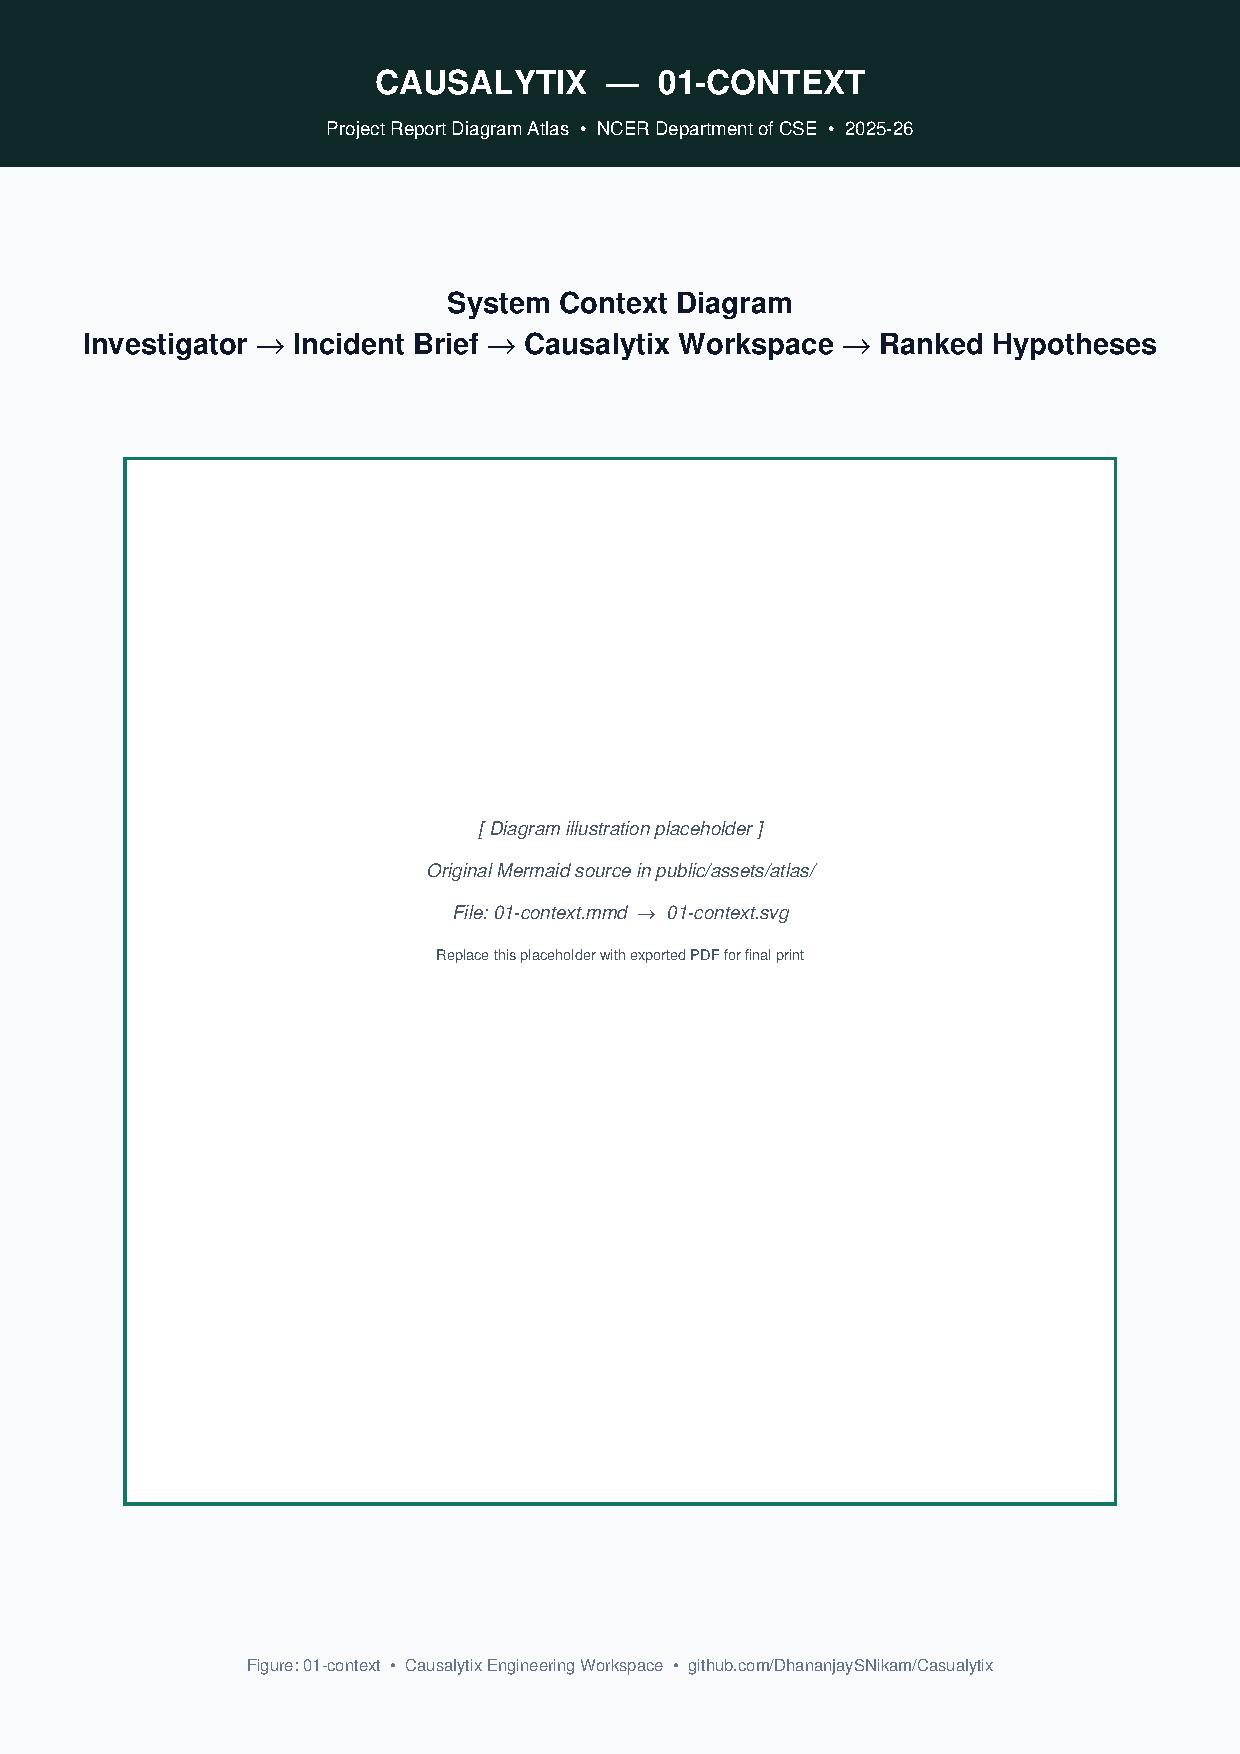
\includegraphics[width=0.92\linewidth]{01-context.pdf}
\caption{System context: investigator supplies brief and evidence; Causalytix returns ranked hypotheses, human verification and reports; optional cloud archive. Original: \texttt{01-context.mmd/svg}.}
\label{fig:context}
\end{figure}

\subsection{Component Architecture}
Figure~\ref{fig:components} decomposes the same-origin application. The FastAPI gateway orchestrates input validation (\texttt{InputBoundary} middleware), passage retrieval, inference and persistence; React renders the workspace. The Supabase path is lazy-loaded and only activates after explicit sign-in and ``Save to cloud''.

\begin{figure}[H]
\centering
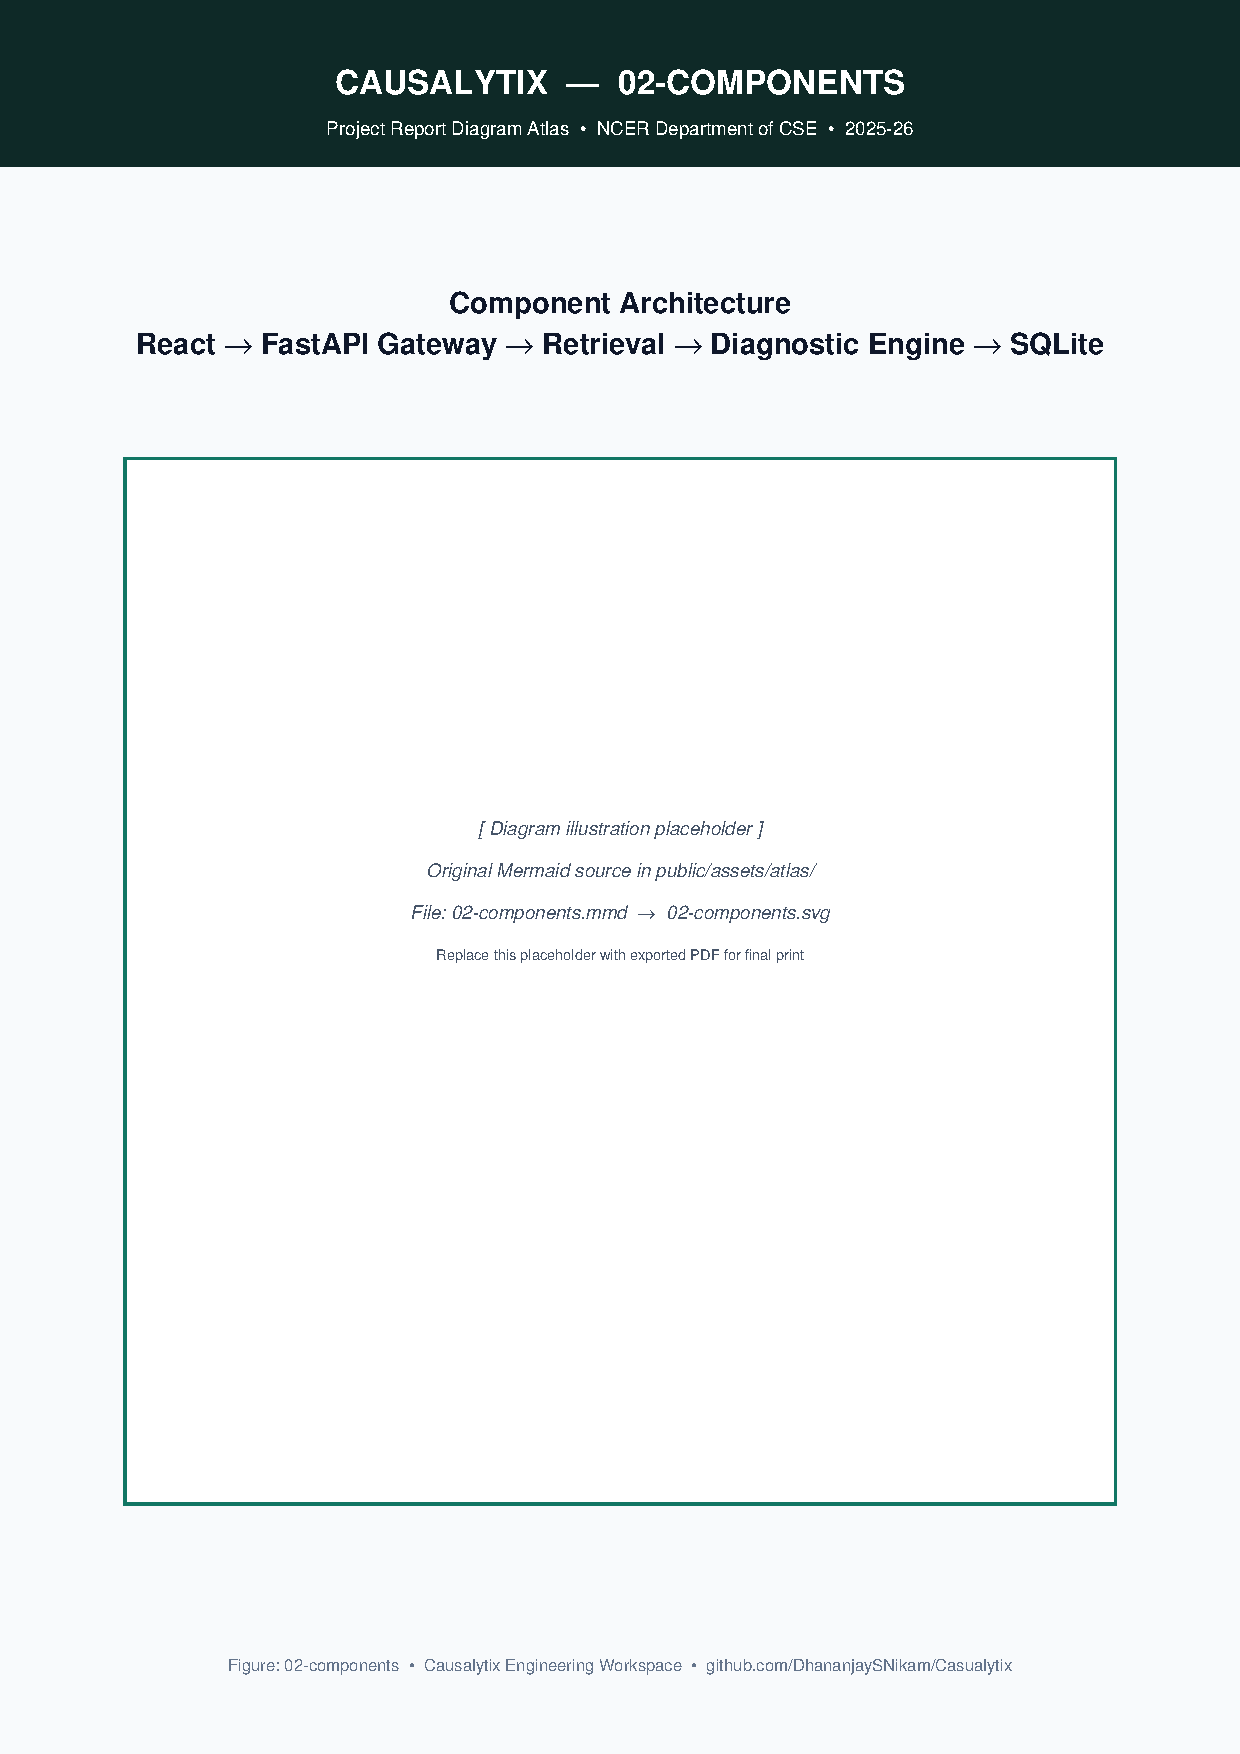
\includegraphics[width=0.92\linewidth]{02-components.pdf}
\caption{Component architecture: React $\leftrightarrow$ FastAPI $\leftrightarrow$ Retrieval $\leftrightarrow$ Diagnostic Engine (Local/LLM) $\leftrightarrow$ SQLite; explicit archive to Supabase Auth/Postgres/pgvector.}
\label{fig:components}
\end{figure}

\subsection{Deployment Boundaries}
Figure~\ref{fig:deployment} clarifies trust boundaries: local SQLite requires no cloud credentials; model inference and cloud archival are separate opt-in paths that send only the brief, retrieved passages and relevant prior-case titles (for LLM) or the full snapshot (for archival) over TLS. Container loopback is not host loopback.

\begin{figure}[H]
\centering
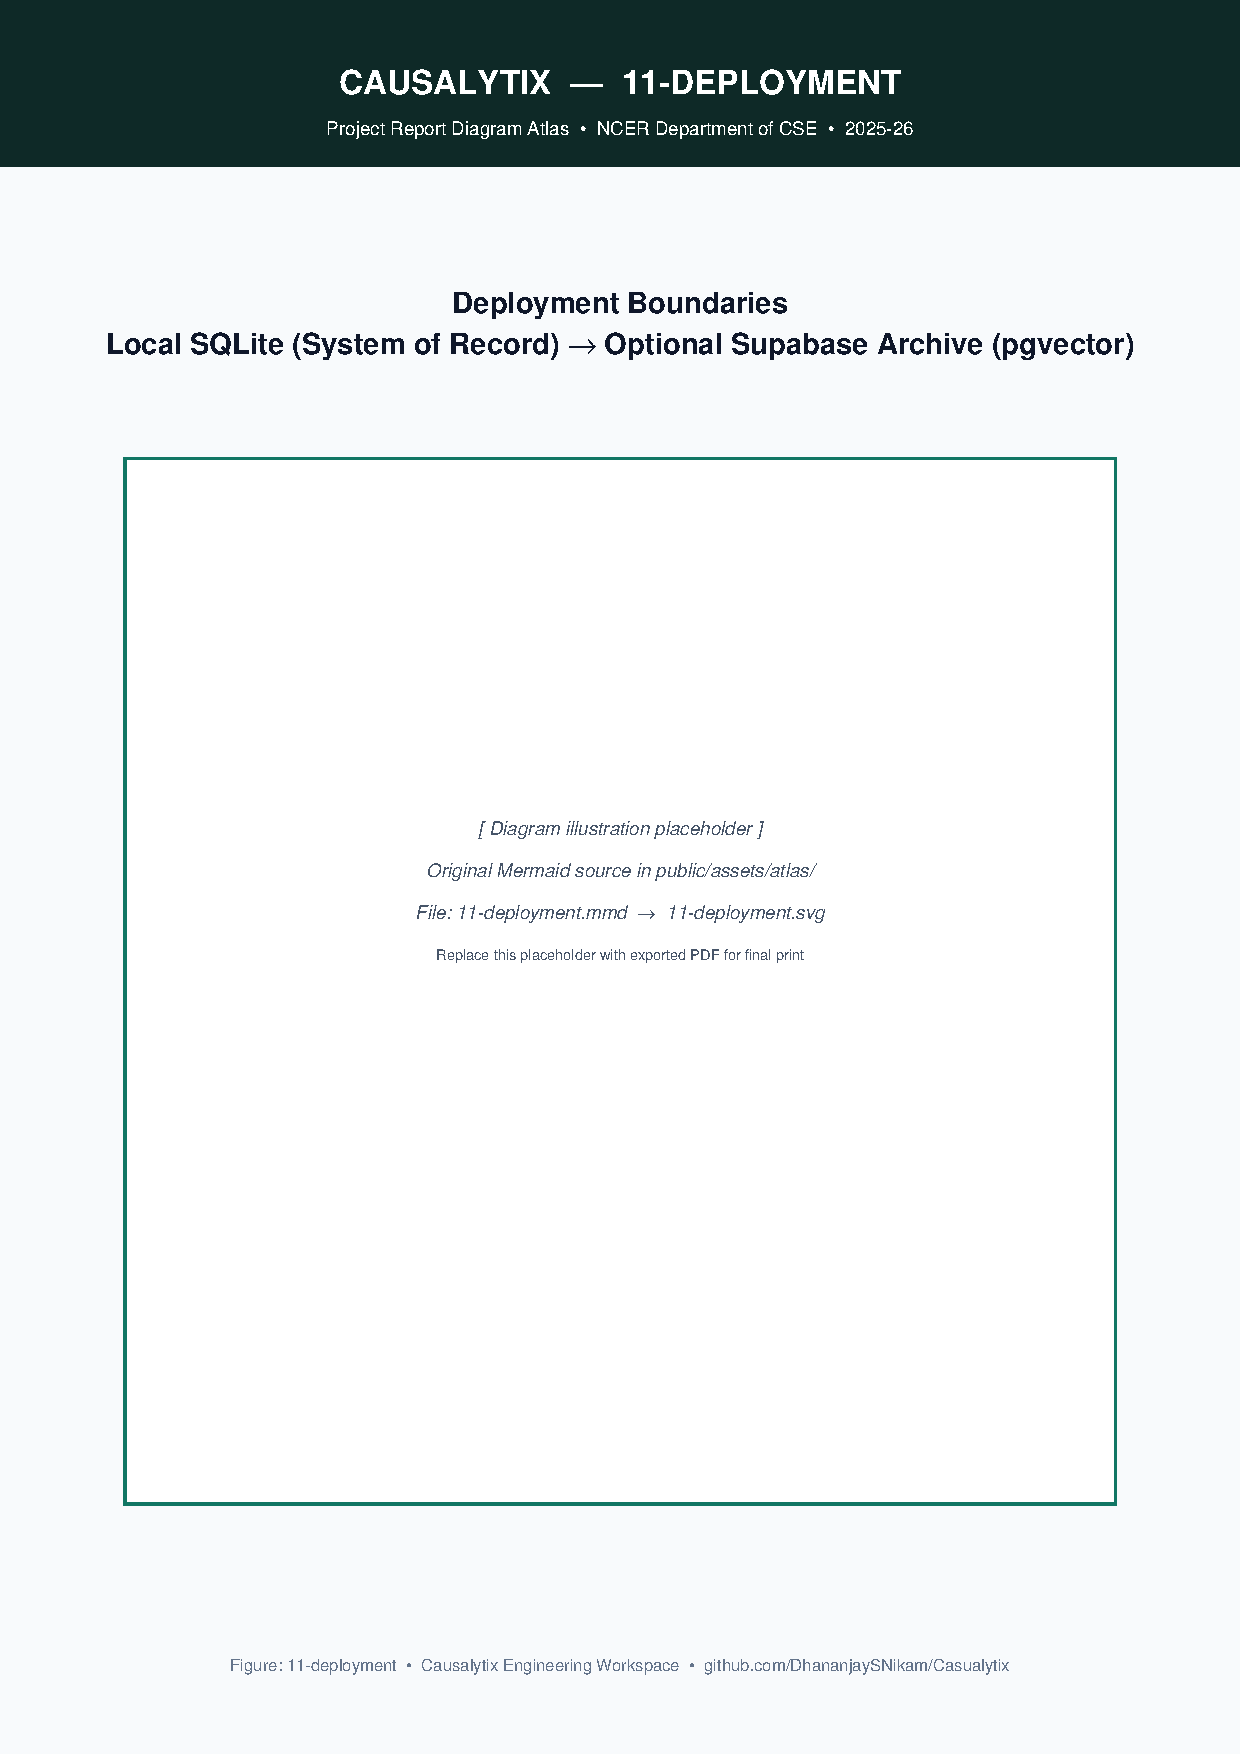
\includegraphics[width=0.88\linewidth]{11-deployment.pdf}
\caption{Deployment boundaries: local-first operation; model endpoint and Supabase are optional and reachable from the container. Original: \texttt{11-deployment.mmd/svg}.}
\label{fig:deployment}
\end{figure}

\subsection{Data Model}
Figure~\ref{fig:erd} shows the entity relationships, mirrored locally and in Supabase (where \texttt{owner\_id} participates in composite foreign keys and RLS policies).

\begin{figure}[H]
\centering
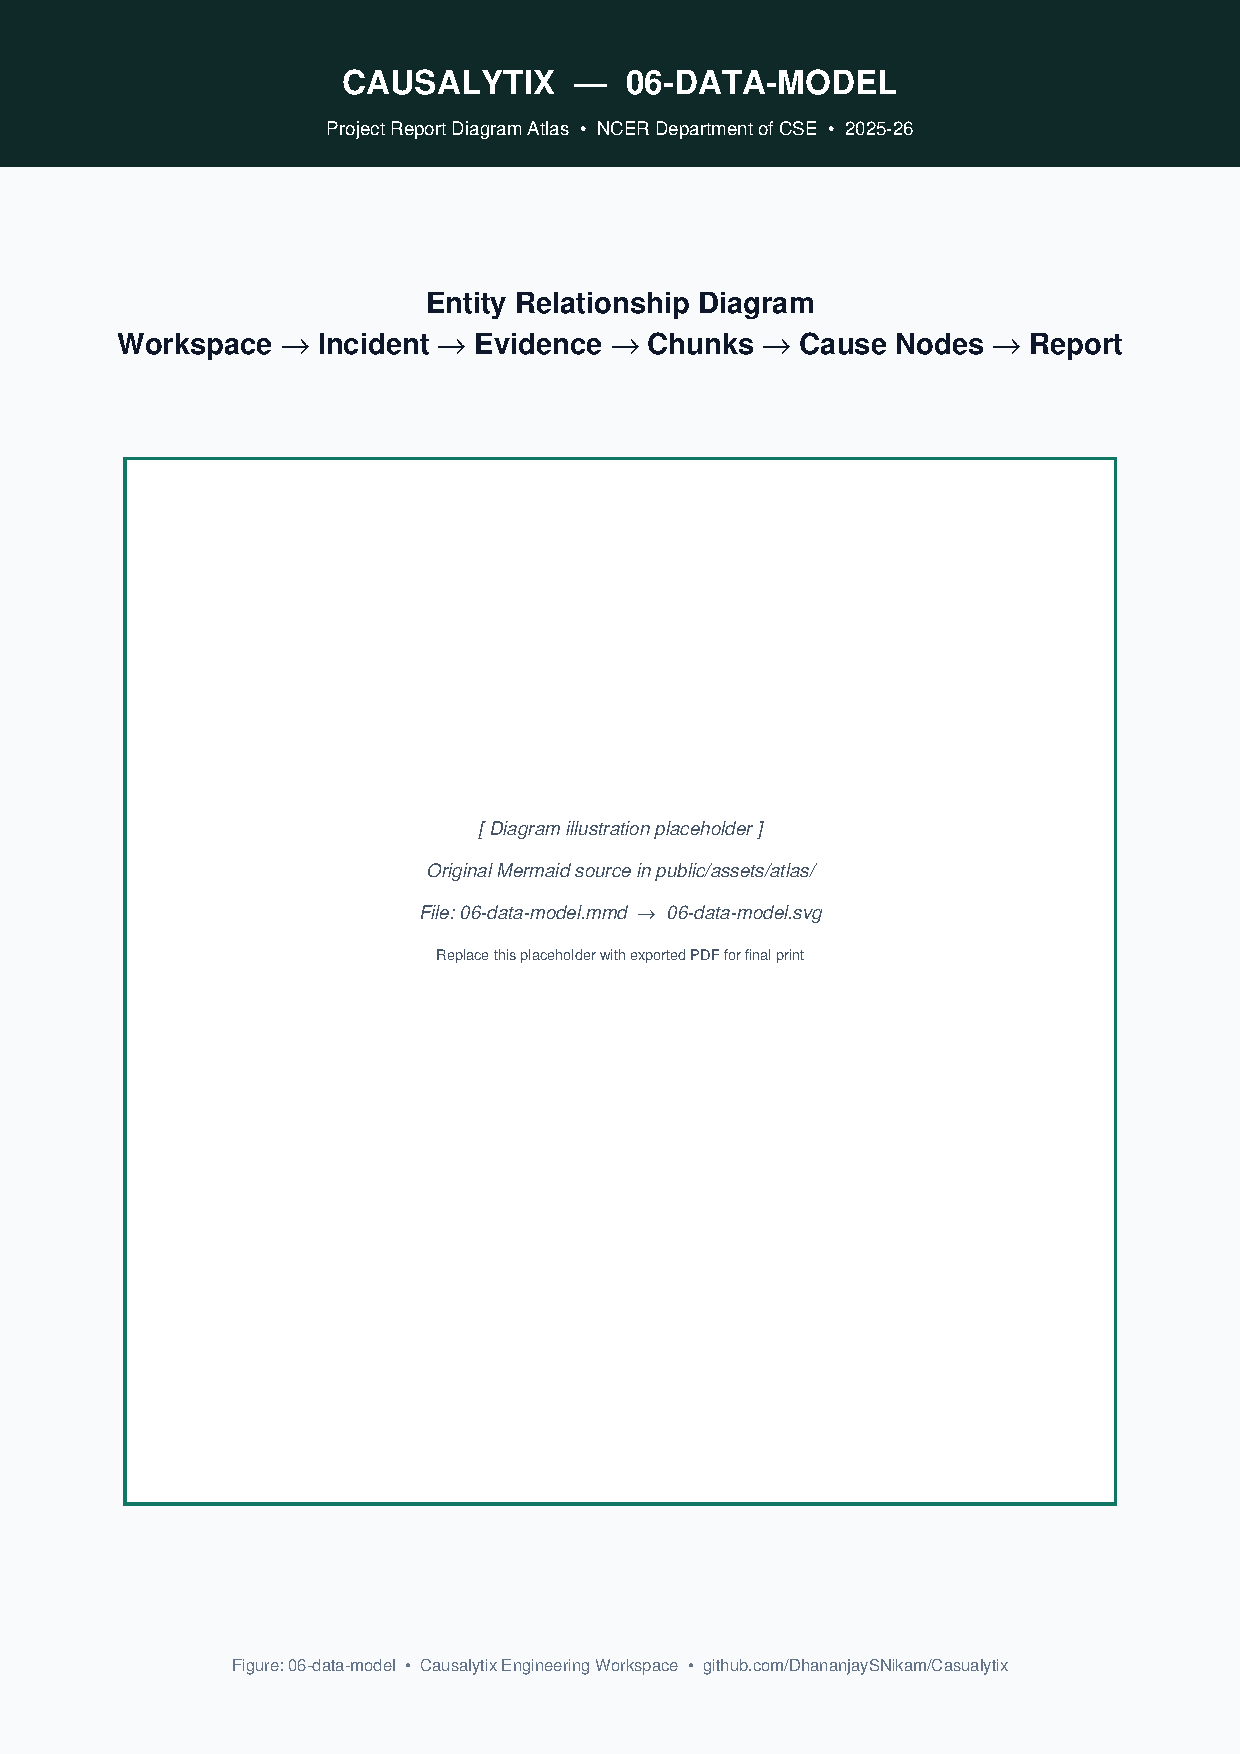
\includegraphics[width=0.92\linewidth]{06-data-model.pdf}
\caption{Entity relationship diagram: Workspace $\rightarrow$ Incident $\rightarrow$ EvidenceDoc $\rightarrow$ DocumentChunk (vector 256) $\rightarrow$ CauseNode $\rightarrow$ RCA Report. Mirrored in Supabase with owner-scoped keys.}
\label{fig:erd}
\end{figure}

Key entities: \texttt{workspaces}, \texttt{incidents} (title, domain, severity, status, brief), \texttt{evidence\_docs} (seq, name, content), \texttt{document\_chunks} (seq, content, embedding[256]), \texttt{cause\_nodes} (branch, depth 0--5, category, label, source), \texttt{rca\_reports} (JSON payload). Cloud tables prefix \texttt{cx\_}.

\section{Process}
\label{sec:process}

\subsection{Nine-Stage Investigation Workflow}
Figure~\ref{fig:workflow} captures the complete lifecycle, including the draft path and the evidence-gap feedback loop that distinguishes Causalytix from linear pipelines.

\begin{figure}[H]
\centering
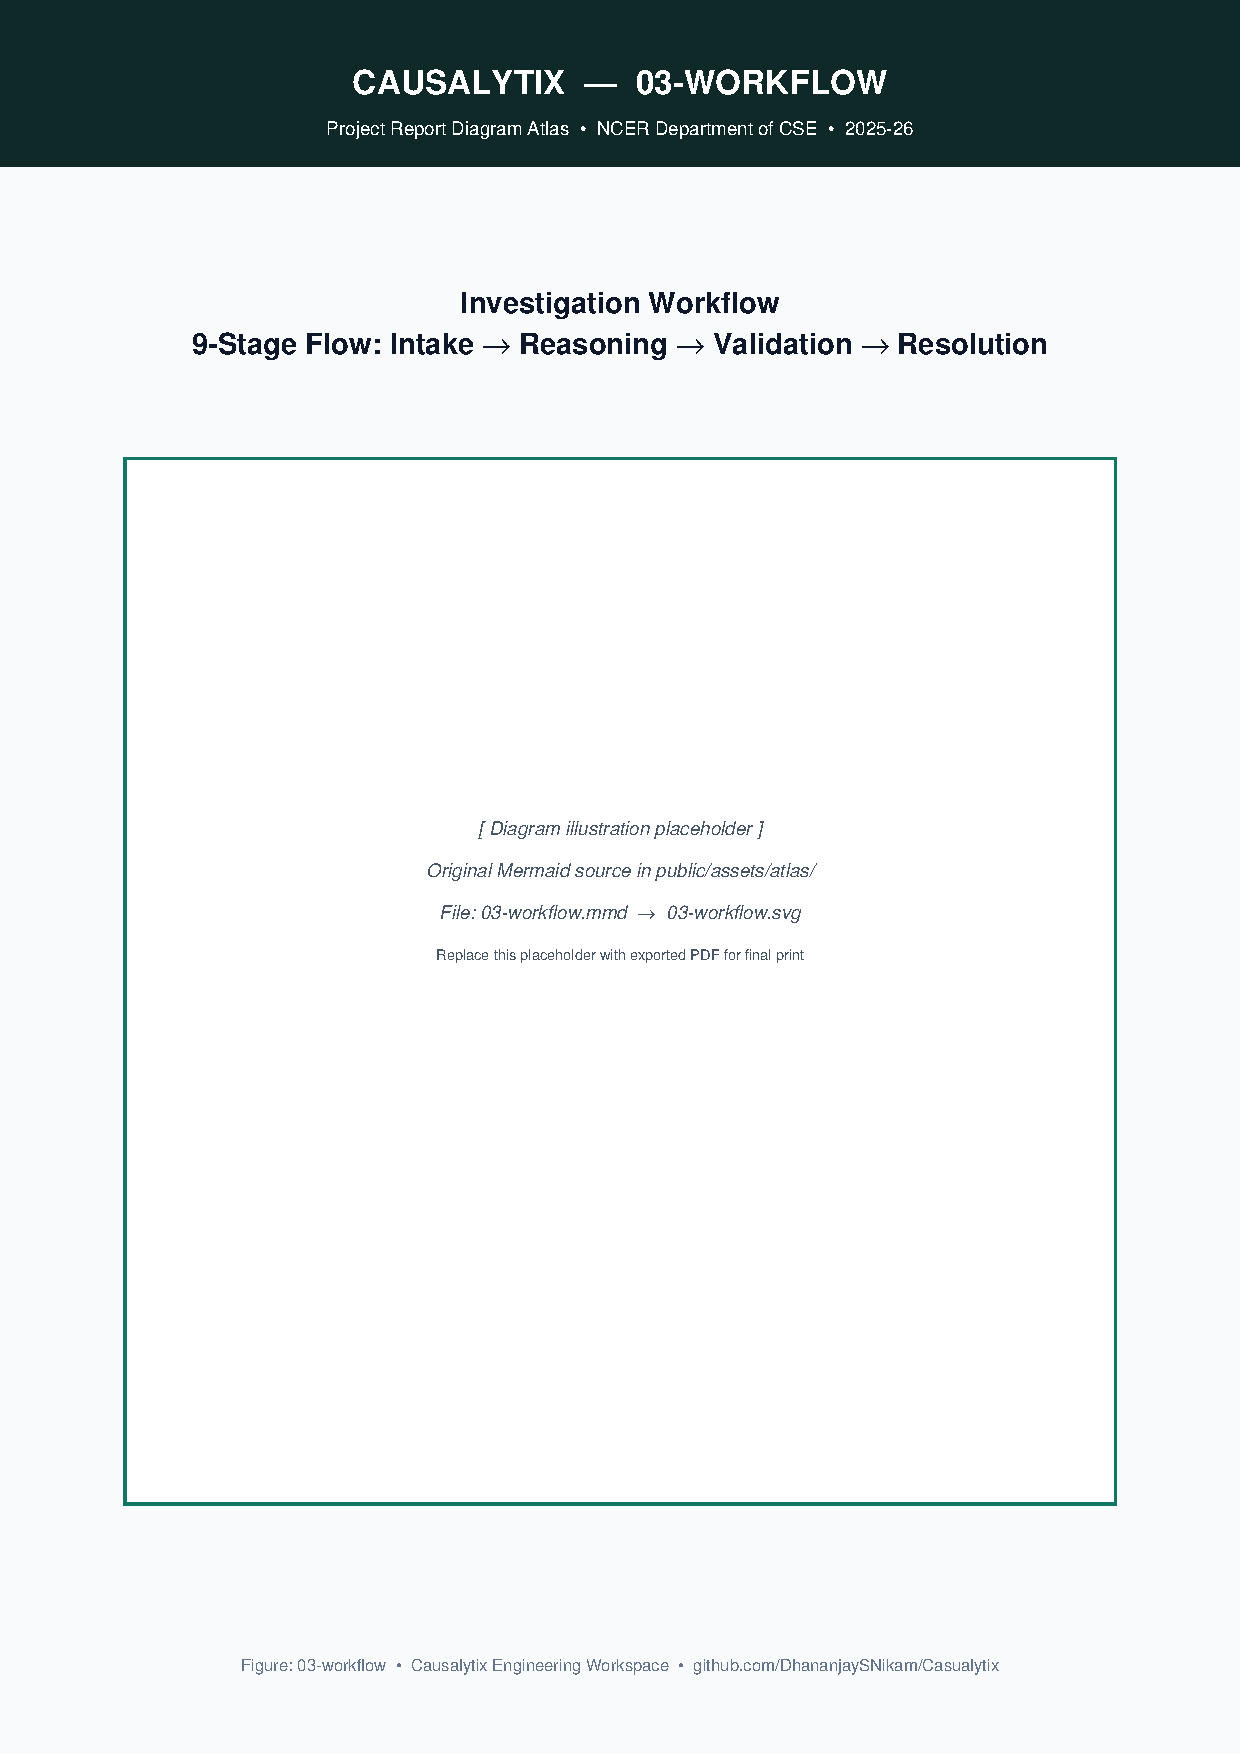
\includegraphics[width=0.96\linewidth]{03-workflow.pdf}
\caption{Investigation workflow: nine stages across Intake, Reasoning, Validation and Resolution, with draft-save and evidence-gap feedback loops. Original: \texttt{03-workflow.mmd/svg}.}
\label{fig:workflow}
\end{figure}

\begin{enumerate}[label=\textbf{\arabic*.},leftmargin=1.6em]
\item \textbf{Problem input (01):} Title, domain (Software/Hardware), observed vs.\ expected, affected system, timeline, severity. Generates a human-readable \texttt{ref} (e.g., \texttt{CX-2025-0042}).
\item \textbf{Evidence intake (02):} Up to six documents per case: file upload or pasted notes; 2~MB/file, 80k chars/item, 30 pages/PDF; text extraction via \texttt{pypdf} for text-layer PDFs; images/CAD/scanned PDFs require a text transcript. Evidence text persisted; binary discarded. Draft can be saved here.
\item \textbf{Generate causes (03):} Gateway selects inference mode (LLM if configured and selected at review step, else local classifier). Local path: multinomial naive Bayes over playbook examples; LLM path: two JSON completions (candidates + impact, then expansions). Pydantic validates shape; failure falls back to local. Up to six candidates, each with category.
\item \textbf{Ishikawa map (04):} Interactive SVG fishbone; each branch is a candidate; clicking a cause highlights its category and rank. Illustrative branches, not confirmed causes, until verified.
\item \textbf{Five Whys (05):} Each candidate expands into five testable Why statements (``Requests may spend most of their time waiting for a connection'' $\rightarrow$ ``Capacity checks may not cover realistic peak workloads''). Each Why is independently evidence-matched.
\item \textbf{Match evidence (06):} For each cause title and each Why text, cosine similarity against the incident's 256-D passage vectors; best match above 0.20 becomes a source (document name, chunk number, excerpt, similarity); otherwise ``Needs evidence'' with a prompt to add evidence.
\item \textbf{Rank causes (07):} $rank = \text{round}(100\times(0.50\cdot\text{evidence}+0.30\cdot\text{impact}+0.20\cdot\text{history}))$; impact mapping Low 0.25/Med 0.50/High 0.75/Critical 1; history counts similar human-confirmed mechanisms in same-domain resolved cases, saturating at 3. Not a calibrated probability.
\item \textbf{Corrective actions (08):} Per candidate: immediate containment (safe, reversible), preventive change (durable fix), verification test (observable pass/fail). Solutions panel separates the three.
\item \textbf{RCA report (09):} Executive summary, ranked causes with sources, 5-Why chains with per-statement provenance, action plan, engineer verification (when resolved), evidence register. Export as paginated PDF or machine-readable JSON.
\end{enumerate}

The evidence-gap loop (06 $\rightarrow$ 02) is deliberate: when a candidate shows ``Needs evidence'', the investigator can add a log or bench note, re-run analysis and observe whether evidence scores change. Draft-save (02 $\dashrightarrow$ Draft) preserves work without generating a report.

\subsection{Evidence Data Flow}
Figure~\ref{fig:evidence} details how a file becomes a citable passage.

\begin{figure}[H]
\centering
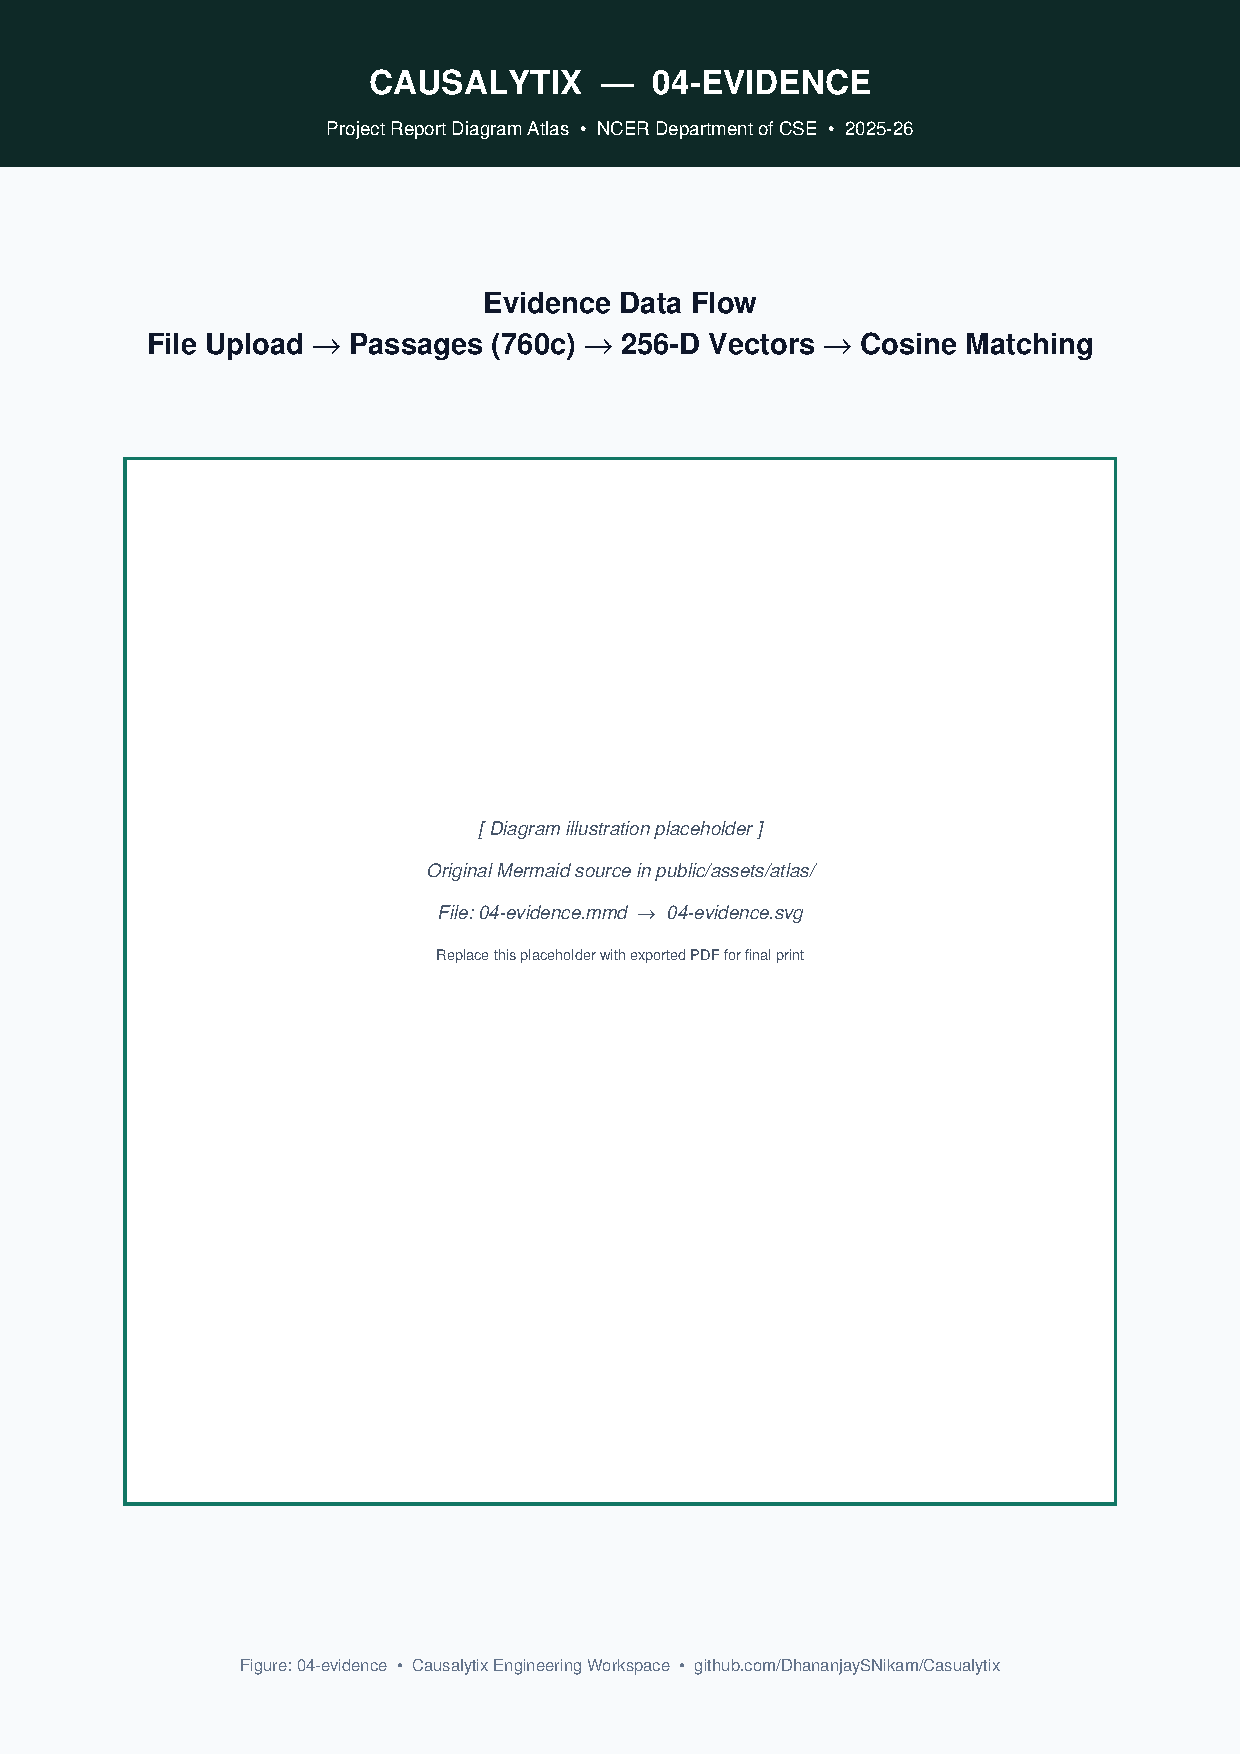
\includegraphics[width=0.88\linewidth]{04-evidence.pdf}
\caption{Evidence data flow: file/paste $\rightarrow$ validation/extraction $\rightarrow$ overlapping passages $\rightarrow$ 256-D vectors $\rightarrow$ passage index $\rightarrow$ cosine matching $\rightarrow$ source or gap. Original: \texttt{04-evidence.mmd/svg}.}
\label{fig:evidence}
\end{figure}

Implementation parameters (from \texttt{backend/engine.py}):

\begin{itemize}
\item Passage length 760 characters, overlap 120, start stride 640; each passage stores \texttt{doc} index, \texttt{index}, \texttt{name}, \texttt{text}, \texttt{embedding}.
\item Tokenization: regex \texttt{[a-z][a-z0-9]+}, lowercase, stop-word removal, domain alias mapping.
\item Vector: log-TF feature hash via BLAKE2s (4-byte digest $\bmod$ 256), L2-normalized, rounded to 6 decimals.
\item Abstention: classifier skips modes with zero vocabulary overlap; support below 0.20 yields evidence gap.
\end{itemize}

\subsection{Analysis Sequence}
Figure~\ref{fig:sequence} shows the runtime collaboration between React, FastAPI, Inference and SQLite.

\begin{figure}[H]
\centering
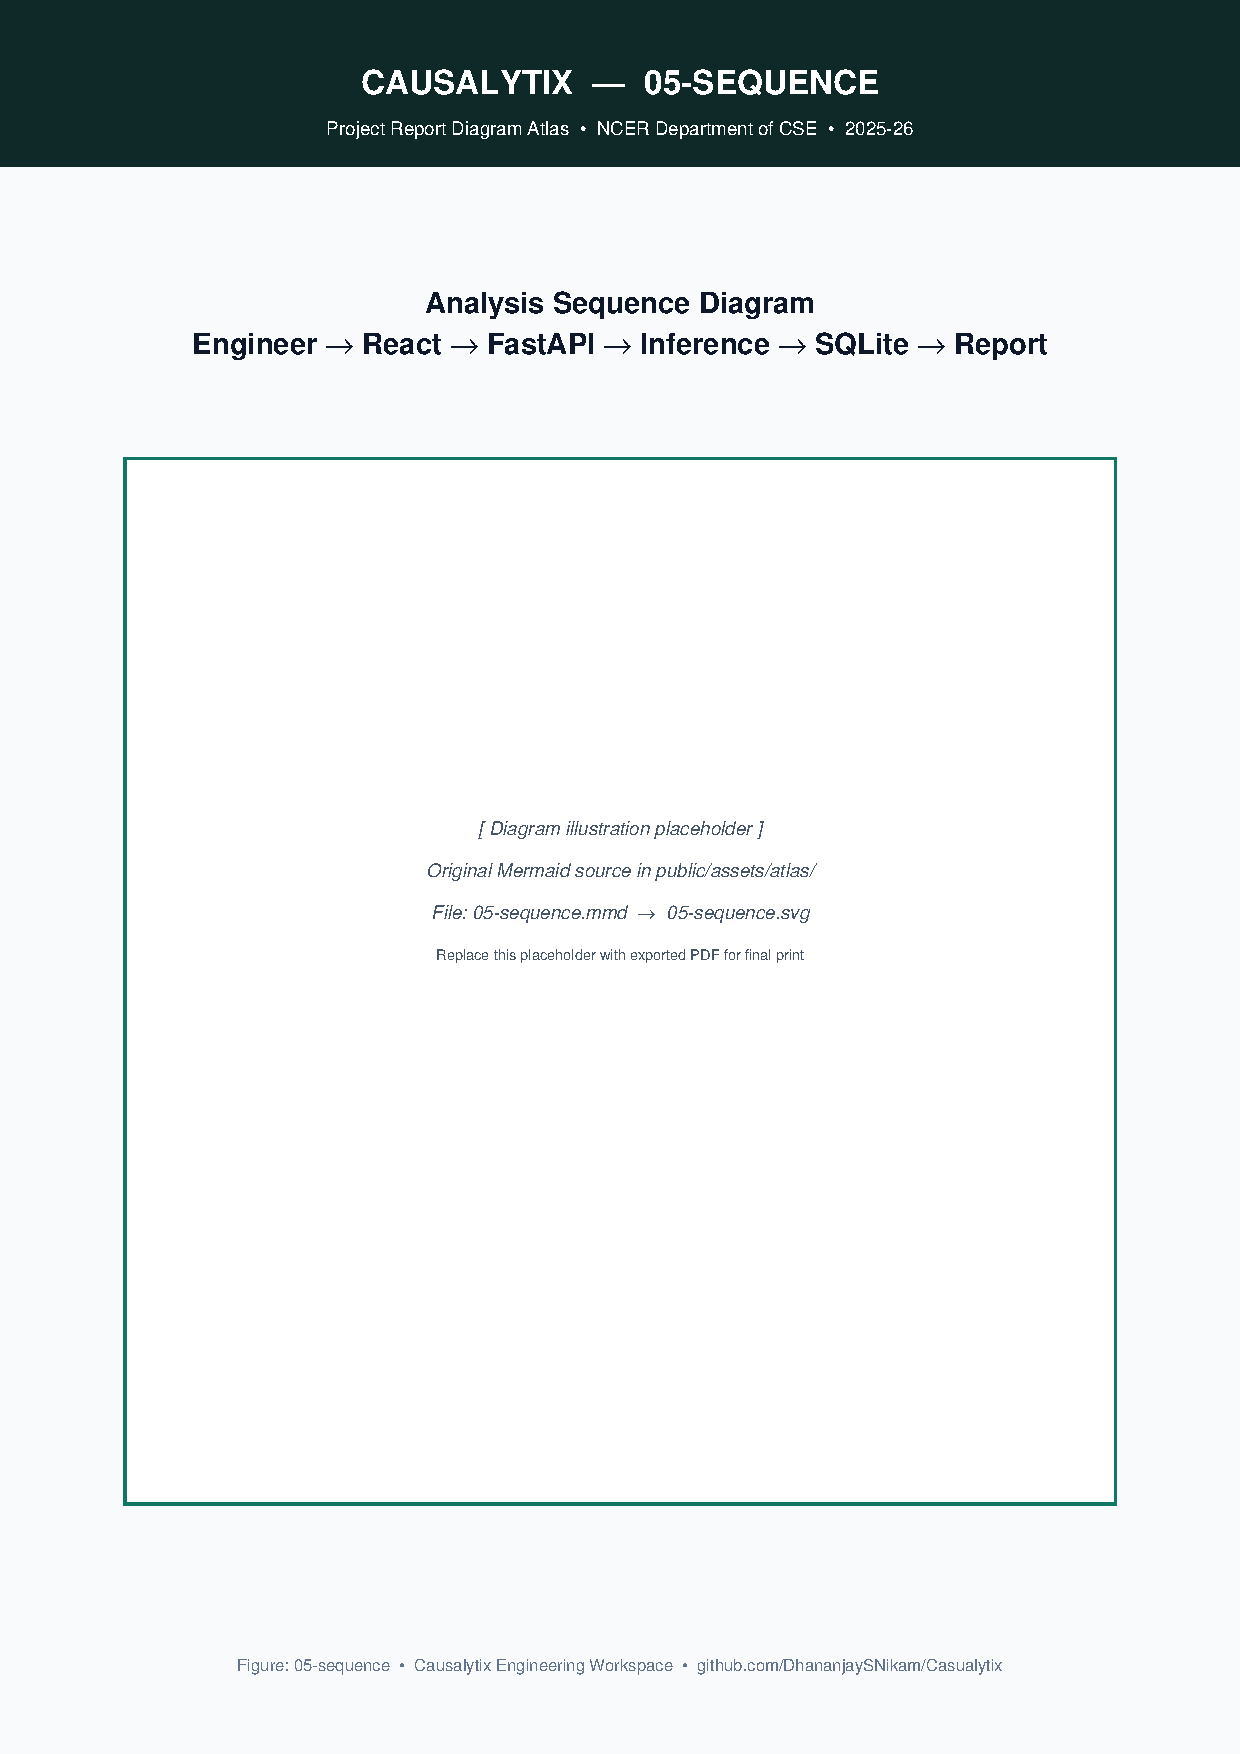
\includegraphics[width=0.88\linewidth]{05-sequence.pdf}
\caption{Analysis sequence: engineer provides brief/evidence; FastAPI reads related resolved cases; inference (LLM two-pass or classifier) returns typed findings; gateway computes sources/ranking and commits.}
\label{fig:sequence}
\end{figure}

The LLM adapter (when enabled) never writes directly to storage; the gateway validates both completions with \texttt{Candidates} and \texttt{Expansions} Pydantic models and then independently computes evidence matches and ranking, ensuring that even a fluent LLM cannot inject an ungrounded score.

\subsection{Case Lifecycle}
Figure~\ref{fig:lifecycle} formalizes state transitions.

\begin{figure}[H]
\centering
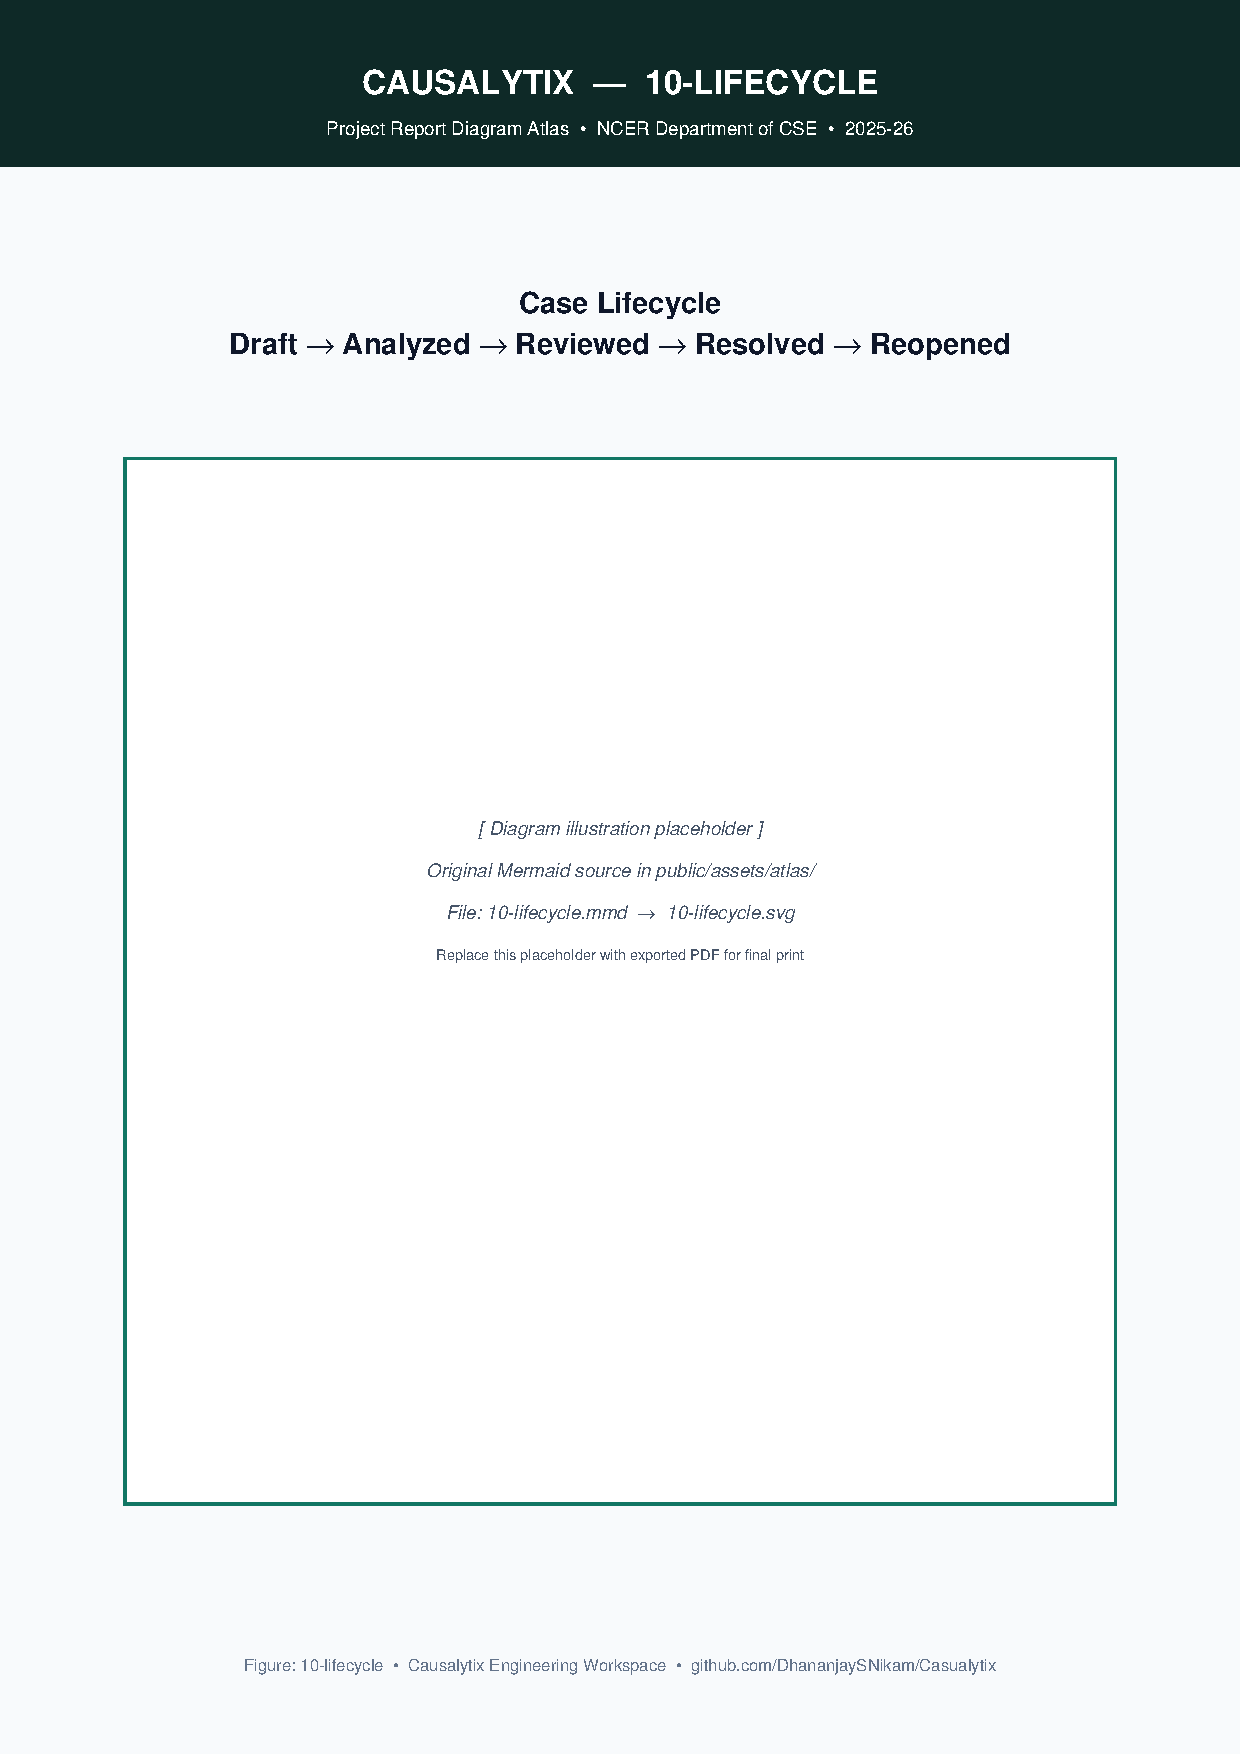
\includegraphics[width=0.85\linewidth]{10-lifecycle.pdf}
\caption{Case lifecycle: drafts can be analyzed, reviewed, resolved (verification gate) and reopened without losing source evidence; editing as draft invalidates prior report.}
\label{fig:lifecycle}
\end{figure}

Rules: \textit{Resolved} requires selecting a confirmed cause and recording the observed test result; that mechanism then counts for future history. Reopening or reanalysis clears active verification. Saving as draft after a report invalidates the prior report (export first).

\section{Block Diagrams and Diagnostic Method Visuals}
\label{sec:block}

This section presents the diagnostic-method figures that appear per investigation.

\subsection{Ishikawa (Fishbone) Mapping}
Figure~\ref{fig:ishikawa} illustrates how candidate branches categorize potential causes. The interactive version lets the engineer click a branch to follow its Why chain.

\begin{figure}[H]
\centering
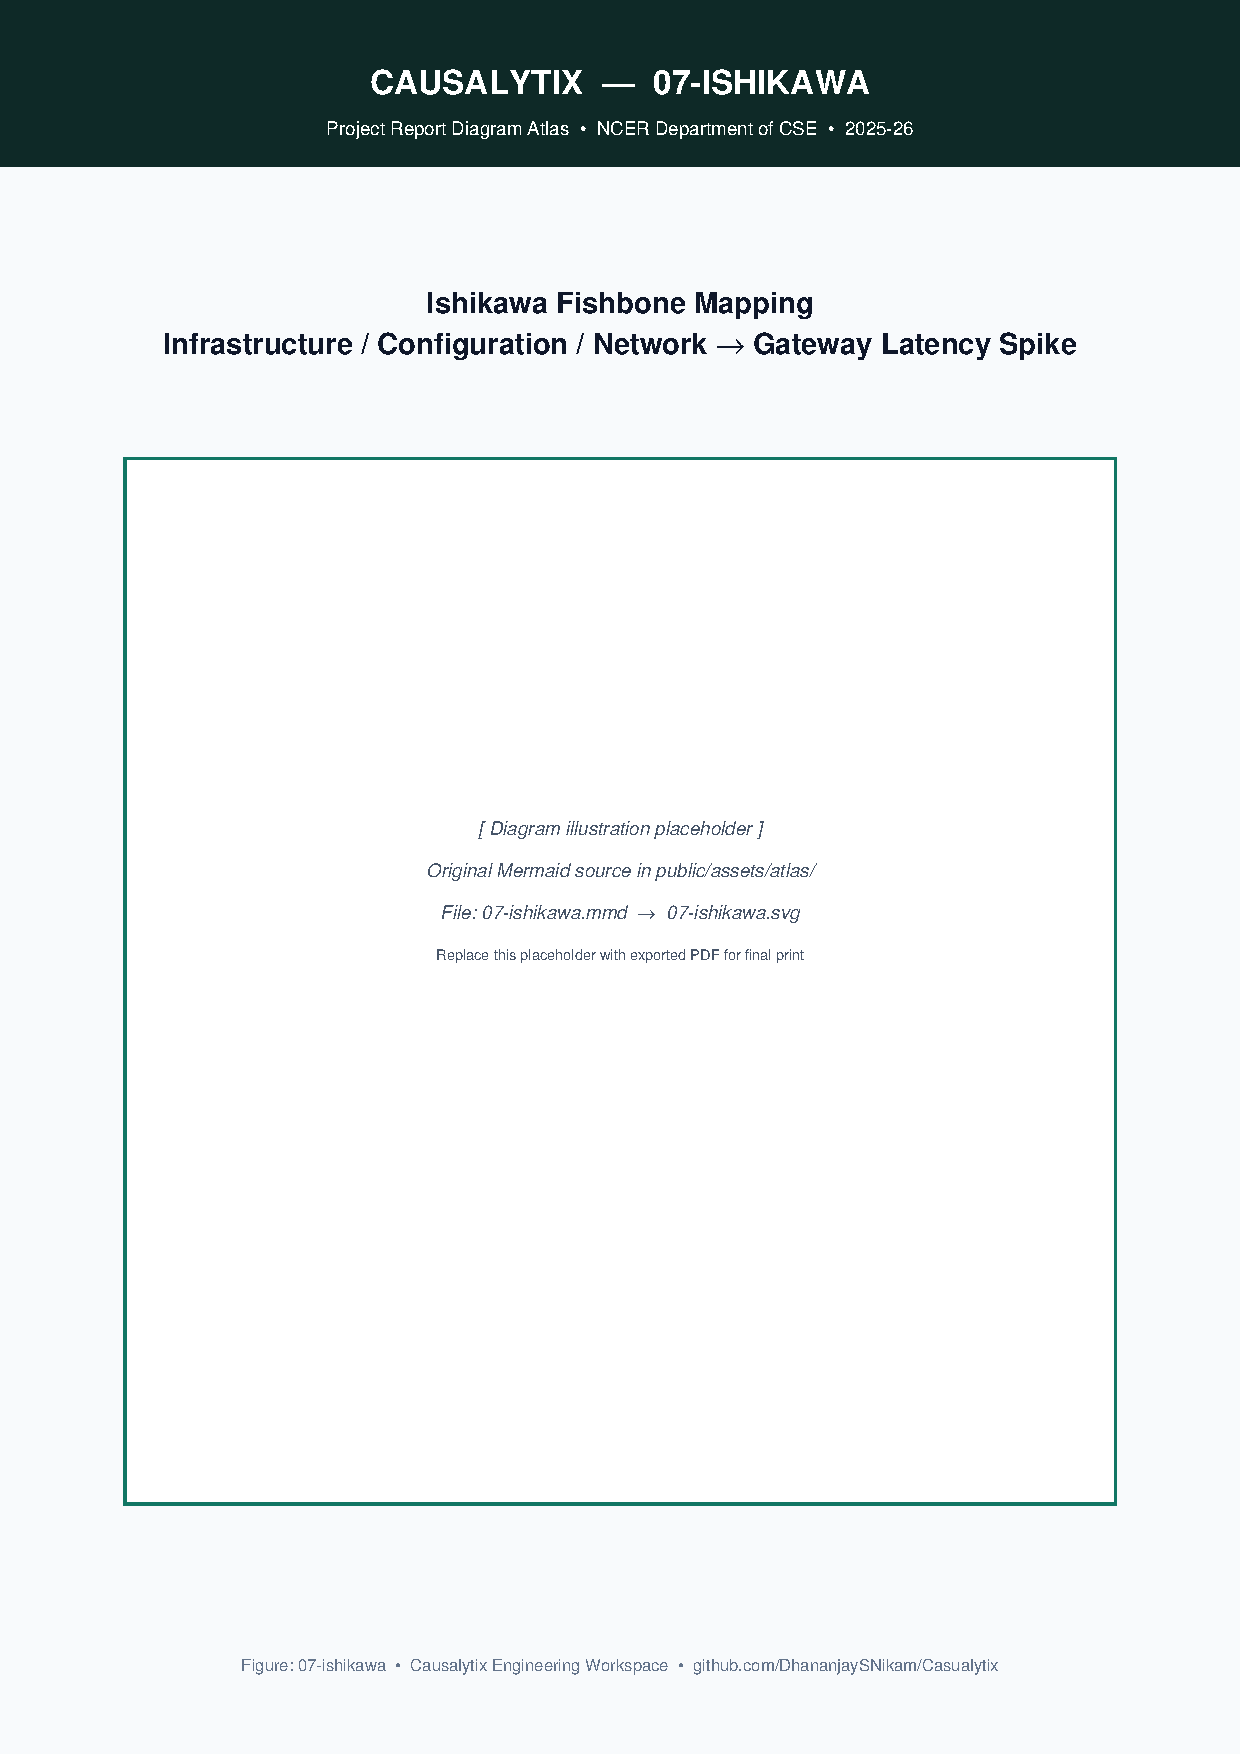
\includegraphics[width=0.88\linewidth]{07-ishikawa.pdf}
\caption{Ishikawa mapping: illustrative branches (Pool saturation $\rightarrow$ Infrastructure, Incompatible release $\rightarrow$ Configuration, Unstable upstream $\rightarrow$ Network) converging on effect (Gateway latency spike). Per-incident map is generated dynamically.}
\label{fig:ishikawa}
\end{figure}

Categories mirror Ishikawa's 4M/6M but adapted to software/hardware: Infrastructure, Configuration, Network, Runtime, Process, Environment, Power, Mechanical, Measurement, etc.

\subsection{5-Why Expansion}
Figure~\ref{fig:why} shows a five-level chain, each step independently evidence-matched. A weak match at any level surfaces as ``Needs evidence'', prompting targeted evidence collection rather than narrative smoothing.

\begin{figure}[H]
\centering
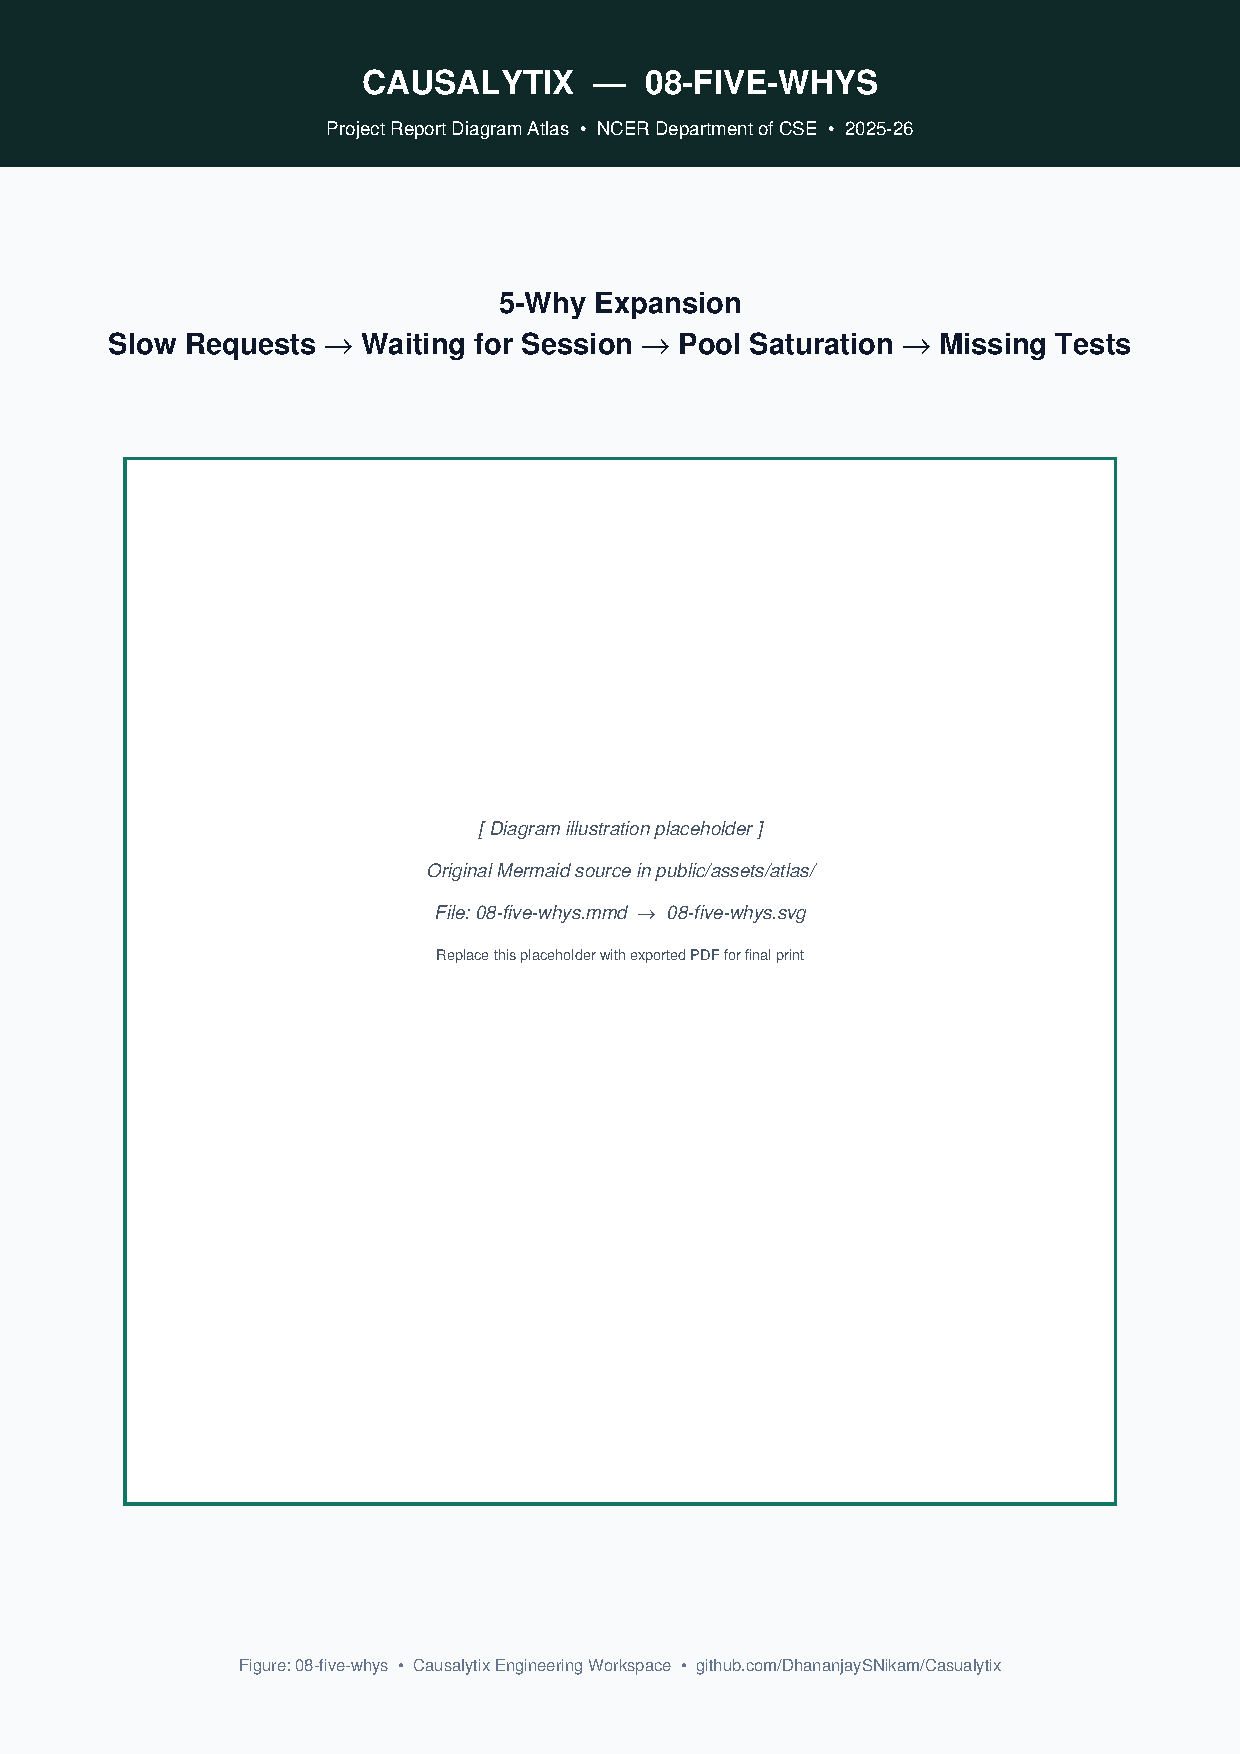
\includegraphics[width=0.82\linewidth]{08-five-whys.pdf}
\caption{5-Why expansion: Slow requests $\rightarrow$ Waiting for session $\rightarrow$ Sessions occupied $\rightarrow$ Long transactions $\rightarrow$ Pool budget mismatch $\rightarrow$ Missing peak tests; pool telemetry comparison leads to verification with controlled workload.}
\label{fig:why}
\end{figure}

\subsection{Root Cause Ranking}
Figure~\ref{fig:ranking} visualizes the weighted sum and the verification decision point.

\begin{figure}[H]
\centering
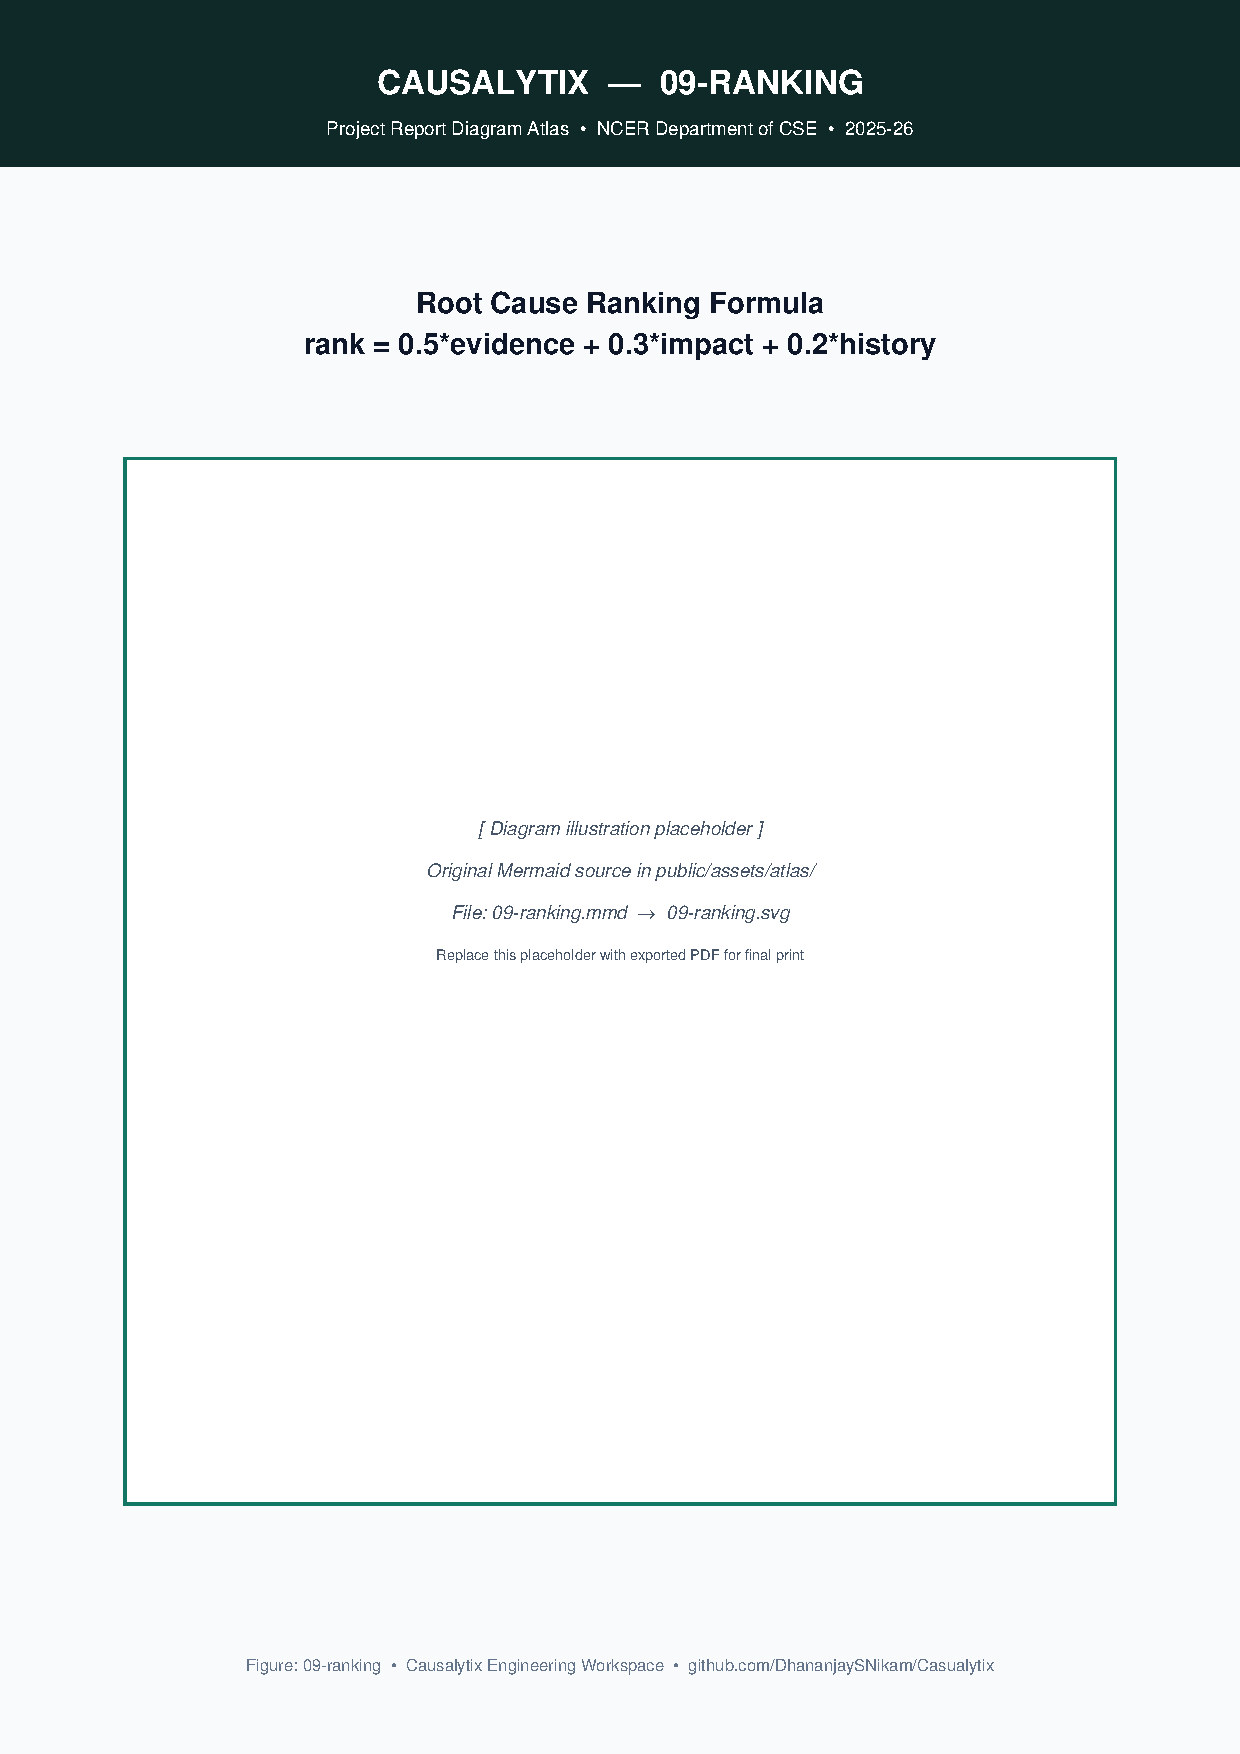
\includegraphics[width=0.86\linewidth]{09-ranking.pdf}
\caption{Root cause ranking: $rank = 0.50\cdot evidence + 0.30\cdot impact + 0.20\cdot history$; verification test determines whether corrective action is confirmed or more evidence is needed.}
\label{fig:ranking}
\end{figure}

The score is intentionally bounded at 100 and rounded; it is a rank, not a probability. Local impact maps Low/Med/High/Critical to 0.25/0.50/0.75/1; LLM impact is validated in $[0,1]$.

\subsection{Summary of Diagrams}
All eleven figures are bundled as a 12-page printable PDF atlas and as individual SVG + Mermaid sources. Table~\ref{tab:figmap} maps each figure to its source file for inclusion in viva slides.

\begin{table}[H]
\centering
\caption{Diagram atlas mapping} \label{tab:figmap}
\begin{tabular}{p{2.2cm} p{4.5cm} p{4cm} p{3.2cm}}
\toprule
\textbf{Fig. ID} & \textbf{Title} & \textbf{Mermaid Source} & \textbf{SVG/PDF}\\
\midrule
01 & System context & \texttt{01-context.mmd} & \texttt{01-context.svg/pdf}\\
02 & Component architecture & \texttt{02-components.mmd} & \texttt{02-components.svg/pdf}\\
03 & Investigation workflow & \texttt{03-workflow.mmd} & \texttt{03-workflow.svg/pdf}\\
04 & Evidence data flow & \texttt{04-evidence.mmd} & \texttt{04-evidence.svg/pdf}\\
05 & Analysis sequence & \texttt{05-sequence.mmd} & \texttt{05-sequence.svg/pdf}\\
06 & Entity relationships & \texttt{06-data-model.mmd} & \texttt{06-data-model.svg/pdf}\\
07 & Ishikawa mapping & \texttt{07-ishikawa.mmd} & \texttt{07-ishikawa.svg/pdf}\\
08 & 5-Why expansion & \texttt{08-five-whys.mmd} & \texttt{08-five-whys.svg/pdf}\\
09 & Root cause ranking & \texttt{09-ranking.mmd} & \texttt{09-ranking.svg/pdf}\\
10 & Case lifecycle & \texttt{10-lifecycle.mmd} & \texttt{10-lifecycle.svg/pdf}\\
11 & Deployment boundaries & \texttt{11-deployment.mmd} & \texttt{11-deployment.svg/pdf}\\
\bottomrule
\end{tabular}
\end{table}

%====================================================================
% CHAPTER 4 - CONCLUSIONS
%====================================================================
\chapter{Conclusions}
\label{ch:conclusions}

\section{Summary of Work Completed}
In Phase-I we designed, implemented and tested \textit{Causalytix}, a local-first engineering workspace that operationalizes root-cause thinking for software and hardware failures. The delivered system demonstrates:

\begin{itemize}
\item A complete nine-stage workflow from problem input to exportable RCA report, with draft-save and evidence-gap feedback loops.
\item Deterministic lexical retrieval (760-char passages, 120-char overlap, 256-D log-TF hash, cosine threshold 0.20) that grounds every cause and every Why in the incident's own evidence.
\item Dual inference: offline naive Bayes classifier with abstention and optional two-pass LLM adapter with Pydantic validation and automatic fallback, sharing a single gateway-computed ranking contract.
\item Transparent ranking $rank = \text{round}(100\times(0.50\cdot evidence+0.30\cdot impact+0.20\cdot history))$ and a human verification gate that governs history influence.
\item Local SQLite WAL system of record and explicit Supabase archival with owner-scoped RLS and pgvector 256, validated by isolated and WASM-based test suites.
\item Eleven report-grade diagrams (context, components, workflow, evidence flow, sequence, ERD, Ishikawa, 5-Whys, ranking, lifecycle, deployment) with Mermaid sources and printable atlas, ready for inclusion in B.E.\ project reports and viva presentations.
\end{itemize}

The eight illustrative starter cases (API gateway latency, memory leak, release mismatch, upstream instability, queue backlog, storage pressure, thermal dissipation, power delivery) allow a new investigator to explore a completed example without supplying evidence, while the seeded database is clearly marked as illustrative and excluded from history counts.

\section{Limitations}
We acknowledge the following Phase-I limitations, each pointing to a concrete Phase-II task:

\begin{enumerate}
\item \textbf{Lexical retrieval limits:} Log-TF hashing can miss deep paraphrase (e.g., ``pool exhausted'' vs.\ ``no available connections''). Dense embeddings (e.g., Sentence-BERT \cite{reimers2019sentencebert}) could improve recall at the cost of model downloads and non-determinism; a hybrid BM25 + dense ensemble \cite{robertson2009probabilistic,izacard2021leveraging} is planned.
\item \textbf{Instrumentation ceiling:} The current evidence cap (6 docs, 30 pages/PDF, 80k chars/item) suits student and lab incidents but not long-running fleet telemetry. Streaming ingestion and OTel native trace support would help \cite{soldani2022anomaly,wang2024comprehensive}.
\item \textbf{Hardware signal depth:} Voltage traces and bench notes are ingested as text excerpts; native time-series alignment (multi-sensor fusion \cite{ran2021robust}, temporal deep learning \cite{angelopoulos2022hardware}) remains future work.
\item \textbf{Evaluation scope:} Tests validate contracts, isolation and fallback, but not MTTR reduction in a live on-call rotation. A controlled user study measuring time-to-hypothesis and report auditability is needed.
\end{enumerate}

\section{Future Scope}
Phase-II will extend Causalytix along four tracks:

\paragraph{(a) Retrieval and inference:} Hybrid lexical + dense retrieval with on-device embedding option, per-domain fine-tuning of the local classifier on anonymized, human-confirmed incidents (with consent), and an evaluation harness comparing ranking against held-out engineer-verified causes.

\paragraph{(b) Collaboration and governance:} Multi-user workspaces with role-based review, comment threads on Why statements, and retention policies for sensitive logs (redaction assist, encrypted SQLite volume).

\paragraph{(c) Hardware depth:} Native CSV time-series viewer for voltage/thermal traces, alignment of reset logs with power traces, and integration with bearing/sensor-fault models \cite{zhang2022intelligent,susto2015machine,jardim2019predictive} for mechatronics projects.

\paragraph{(d) Deployment and pedagogy:} Helm chart for Kubernetes, OIDC for campus deployments, and a tutorial library mapping each starter case to its Ishikawa/5-Why interpretation, enabling use as a teaching lab for RCA.

We aim to publish the workspace and a Phase-II evaluation as an open-access tool paper, contributing the anonymized playbook taxonomy and the verification-gated history mechanism back to the AIOps community \cite{remil2024aiops,chen2024rcacopilot}.

%====================================================================
% REFERENCES
%====================================================================
\cleardoublepage
\addcontentsline{toc}{chapter}{References}
\bibliographystyle{IEEEtran}
\bibliography{references}

%====================================================================
% ANNEXURE A
%====================================================================
\chapter*{ANNEXURE A}
\addcontentsline{toc}{chapter}{ANNEXURE A}

\section*{I.\ Paper Published / Paper Acceptance}
\addcontentsline{toc}{section}{I.\ Paper Published / Paper Acceptance}

\begin{center}
\begin{tabular}{|p{14cm}|}
\hline
\textit{Paper title, venue, status and acceptance proof to be inserted here.}\\
\textit{Target: Tool paper on Causalytix (Phase-II evaluation) for submission to} \\
\textit{ACM SIGOPS OSR / IEEE ICSE-SEIP / FSE Companion (tool track).}\\
\textit{Attach acceptance email / publication certificate when available.}\\
\\
\blankline[14cm] \\
\\
\hline
\end{tabular}
\end{center}

\section*{II.\ Intellectual Property Rights (IPR)}
\addcontentsline{toc}{section}{II.\ Intellectual Property Rights (IPR)}

\begin{center}
\begin{tabular}{|p{14cm}|}
\hline
\textit{IPR filing details (if any) to be inserted here.}\\
\textit{Codebase licensed under MIT (see LICENSE file) at}\\
\textit{https://github.com/DhananjaySNikam/Casualytix .}\\
\textit{Diagram atlas and report template are original work of the project team;}\\
\textit{third-party assets (React, FastAPI, ReportLab, fonts Lucide/Inter/Space Grotesk/IBM Plex Mono) are under their respective permissive licenses (MIT, OFL) as documented in public/assets/licenses/.}\\
\\
\textit{If applying for copyright / patent, attach filing receipt.}\\
\\
\blankline[14cm] \\
\\
\hline
\end{tabular}
\end{center}

\vspace{0.5cm}
\noindent\small \textit{Note: Author names, PRN, guide name and coordinator signature blocks are intentionally left blank in this Phase-I template for manual completion before submission, as per department instructions. College name, department header/footer and formatting (A4, margins, Times 12pt, 1.5 spacing, header/footer, page numbering) conform to Project Report Guidelines 2025--26.}

\end{document}
